\documentclass{article}
\usepackage[margin=1in]{geometry}
\usepackage{graphicx}
\usepackage{enumitem}
\usepackage[toc,page]{appendix}
\usepackage{amsfonts}
\usepackage{amsmath}
\usepackage{amsthm}
\usepackage{commath}
\usepackage{color}

\title{FLASH Orchestration System Design}

% No automatic indenting
\setlength\parindent{0pt}

% Set spacing between items in itemize/enumerate
\setlist{itemsep=1pt}

\newcommand{\N}                 {{\mathbb N}}
\newcommand{\Z}                 {{\mathbb Z}}
\newcommand{\Q}                 {{\mathbb Q}}
\newcommand{\R}                 {{\mathbb R}}
\newcommand{\C}                 {{\mathbb C}}
\newcommand{\F}                 {{\mathbb F}}

\newcommand{\SetuptimeParam}[1] {\textcolor{red}{#1}}
\newcommand{\RuntimeParam}[1]   {\textcolor{blue}{#1}}
\newcommand{\ComposerKey}[1]    {\textcolor{cyan}{#1}}

\newcommand{\TeamStarting}      {\textsc{TeamStarting}}
\newcommand{\TeamIdle}          {\textsc{TeamIdle}}
\newcommand{\TeamRunningOpen}   {\textsc{TeamRunningOpen}}
\newcommand{\TeamRunningClosed} {\textsc{TeamRunningClosed}}
\newcommand{\TeamRunningNoMoreWork} {\textsc{TeamRunningNoMoreWork}}
\newcommand{\TeamTerminating}   {\textsc{TeamTerminating}}

\newcommand{\ThreadStarting}    {\textsc{ThreadStarting}}
\newcommand{\ThreadIdle}        {\textsc{ThreadIdle}}
\newcommand{\ThreadComputing}   {\textsc{ThreadComputing}}
\newcommand{\ThreadWaiting}     {\textsc{ThreadWaiting}}
\newcommand{\ThreadTerminating} {\textsc{ThreadTerminating}}

\begin{document}

% Setup numbered/referentiable environment for requirements
\theoremstyle{definition} % No italics or spaces
\newtheorem{req}{Req}[section]
\newtheorem{spec}{Spec}[section]

\maketitle

%%%%%----- ORCHESTRATION SYSTEM EXECUTIVE SUMMARY -----%%%%%
\section{Executive Summary}
This document is intended to be a static snapshot of the FLASH5 development
team's understanding of the design and requirements associated with the
Orchestration System that is under development for inclusion in FLASH5.  This
document has been informed by discussions within the group and with
collaborators as well as through some prototyping of the Orchestration Runtime
in FLASH5 with the \texttt{simpleUnsplit} Hydro implementation.  However, as a
static document, the contents here will likely not be updated as our
understanding of the design of this system improves with implementation of the
system.\\

The \textbf{orchestration system} is a performance portability system that will
allow FLASH5 to run in CPU-only mode or to make good, efficient use of resources
when run on heterogeneous platforms on which the notion of host-to-device
offloading exists. The orchestration system is comprised of
\begin{enumerate}
\item{an offline \textbf{task scheduler} that}
    \begin{itemize}
    \item{reads in metadata orchestration files for all kernels, all tasks, all
    operations, and for the simulation,}
    \item{reads in a general, high-level representation of each operation,}
    \item{creates a kernel graph of all kernels to be executed at each time step,}
    \item{attempts to optimize resource use for the given platform using the
    above information by fusing tasks and bundling tasks for
    execution with the orchestration runtime, and}
    \item{writes to \texttt{Driver\_evolveFlash} the bundles as a sequence of runtime executions (one task
    bundle per runtime execution) in an order that preserves dependencies,}
    \end{itemize}
\item{an offline \textbf{code generator} that generates Fortran code optimized
for the given platform and that serves as the code layer that patches
orchestration runtime execution (\texttt{Driver\_evolveFlash}) with base Fortran
code that executes kernels and tasks on data defined on individual domain tiles,
and}
\item{an \textbf{orchestration runtime} that}
    \begin{itemize}
    \item{is invoked for each task bundle,}
    \item{exposes to the client code multiple different mappings of tasks in a
    bundle to hardware resources\footnote{It is the responsibility of the task
    scheduler to pick a mapping that will maximize efficient use of parallel
    computational resources without violating intertask dependencies.},}
    \item{allows for balanced, dynamic loading of host processors,}
    \item{knows where and how to efficiently transfer data,}
    \item{manages memory and device resources to prevent incorrect access and
    promote efficient resource use, and}
    \item{leaves data in the appropriate memory resource.}
    \end{itemize}
\end{enumerate}
The orchestration runtime is needed to expose the hierarchy of parallelism of a
given platform's hardware; the collection of offline tools, to adapt the
software to the runtime so that the software can take advantage of the exposed
parallelism.  The division of labor between multiple tools is made not only to
achieve good encapsulation and modularity, but also to ensure that no single
tool is too complex or requires too much intelligence.  Refer to
Table~\ref{tab:ParallelHierarchy} for a detailed view of the aforementioned
hierarchy.\\

Our design is forward-looking in the sense that we hope our
design will not preclude running on future heterogeneous platforms in which
multiple distinct devices including the host might exist in the same chip
package (higher NUMA complexity) or in which multiple distinct devices including
the host might share the same physical memory package (altering the role of data
transport in a single simulation).  Specifically, our three-levels of
future-proofing consider that the design must allow for
\begin{itemize}
\item{One host + many accelerators (offloading),}
\item{tighter coupling between host \& host devices
(physically-unified memory / GPU and CPU have the same memory) --- memory
barriers to manage resource access dependencies.  NUMA effects (e.g. GPU and CPU
on same chip) would require that user can dictate mapping of tasks onto HW.
Same memory could mean that data movements become unnecessary.  This last point
seems hard.}
\item{Runtime adaptiveness/forecasting --- this is the interface between the
runtime and the offline tools --- we have the Orchestration runtime public
interface that dictates task bundles and on the other side a task graph that is
executed in task bundles on the runtime.}
\end{itemize}

We emphasize that not only should the design/implementation allow for us to
account for such future developments, but also adjusting the
design/implementation should be scalable such that updating the software to use
new or different hardware features should be easy and result in maintainable
code.

\begin{table}[!t]
\label{tab:ParallelHierarchy}
\caption{The hierarchy of parallelism that the Orchestration System design
should expose and capitalize on.  The table is ordered from coarsest parallelism
(top) to finest.  Refer to Section~\ref{sec:Definitions} for definitions of
terms that appear in the table and Section~\ref{sec:Runtime} for more
information regarding Thread Teams.  \textcolor{red}{Should pipelining within a
runtime configuration be added to this table?}}

\begin{center}

\begin{tabular}{|p{1.1in}|c|c|c|p{2.25in}|}
\hline
Title & Parallelism & HW Scope & SW Scope & Description\\
\hline
\hline
MPI                              & Data Parallel & Machine & Domain    & Domain decomposition into blocks\\
\hline
Block Iterator                   & Asynchrony    & Machine & Time step & Overlay guardcell fill communication with computation\\
\hline
Task Bundles with concurrency    & Task Parallel & Node    & Time step & Run independent tasks concurrently across all node resources\\
\hline
Task Bundles with work splitting & Data Parallel & Node    & Time step & Use different devices to apply single task to assigned blocks\\ 
\hline
Thread Teams                     & Data Parallel & Node    & Task      & Apply a single task to assigned blocks using host and optionally accelerators\\
\hline
Device Kernels                   & Data Parallel & Device  & Kernel    & Oversubscribe device with kernels to hide latencies\\
\hline
Device HW                        & Data Parallel & Device  & Comp.     & Schedule individual computations across processing units in device\\
\hline
\end{tabular}

\end{center}
\end{table}

%%%%%----- ORCHESTRATION SYSTEM DEFINITIONS & OVERVIEW -----%%%%%
\section{Definitions \& General Design}
\label{sec:Definitions}
The term \textbf{unit} is used as per the normal Flash definition.  In
particular, we would like to emphasize that a unit can contain
\begin{itemize}
\item{standalone public routines that function as helper routines,}
\item{standalone private routines that function as helper routines, and}
\item{routines that execute a high-level computation or action.}
\end{itemize}

This latter class of routines are referred to as \textbf{operations} and
\textit{typically} are routines that
\begin{itemize}
\item{are called by the \texttt{Driver\_evolveFlash} routine,}
\item{outline at a high-level the steps of a computation, and}
\item{execute the computation on all tiles in the domain by using the tile
iterator at least once.}
\end{itemize}
An example of an
operation is the updating of the solution at a single time step by the Hydro
unit and its highest-level representation is the code in \texttt{Hydro.F90}.
The Gravity unit has many different operations including ... and solving for the
gravitational potential (\texttt{Gravity\_potential.F90}).  Note that operations
can call operations.  For instance, the Hydro step operation may call the
Gravity unit's operation that solves for the gravitational potential.\\

In this document the units of heavy-computation work that are written in the
form of one or more nested loops are sensibly referred to as \textbf{loop
nests}.  Each distinct set of code that is run on a device as a single unit of
computation is known as a \textbf{kernel}.  In general, each kernel will consist
of one loop nest and the iteration space of the loop nest will be over a section
of the index space of the domain (\textit{i.e.} a set of cells or faces located
in a contiguous, rectangular region of the discretization of the domain).  This
is advantageous as we hope that the computational load of the loop nest will be
sufficiently large for amortizing the cost of transferring data and launching
the kernel on the device.  Note that in some cases, it might be reasonable to
group together lines of code that do not contain a single loop nest.  For
instance, such kernels might be called to set the values of variables in the
device memory so that we can avoid the potentially more expensive alternative of
setting the variables in the host memory and transferring the values to the device
memory.\\

\textbf{Tasks} are the smallest unit of work that can be executed by the
Orchestration runtime and each task may consist of kernel launches interleaved
with code blocks to be run on the host.  In its simplest form, a task may
consist of code that does not loop over tiles and such tasks are defined as
\textbf{auxiliary tasks}.  Though relatively simple, these tasks may also launch
non-trivial kernels.  For instance an auxiliary task may launch a kernel that
populates via a loop nest an array variable allocated in device memory
(\textit{e.g.} compute the speed of sound across the cells in a region of the
domain).  Tasks that perform one loop over a subset of tiles in the domain are
defined as \textbf{work tasks}.  Note that the design of the runtime does not
allow for tasks that execute more than one tile iteration loop.\\

An important aspect of the runtime is that each execution of the runtime exposes
parallelism in at least two different ways (Table~\ref{tab:ParallelHierarchy}).
The first level of parallelism can be exploited when certain Grid unit
operations that involve global data communication can be overlaid asynchronously
with one or more subsequent work tasks.  This type of parallelism is exposed
through the Grid unit's iterator and therefore depends on whether a particular
implementation of the Grid unit supports it and on which global communication
operations it supports.  For example, the Paramesh implementation of the Grid
unit does not have asynchronous tile iterators, but AMReX implementation of the
Grid unit will allow overlaying the filling of guardcells with execution of work
tasks.\\

\begin{figure}[!ht]
\begin{center}
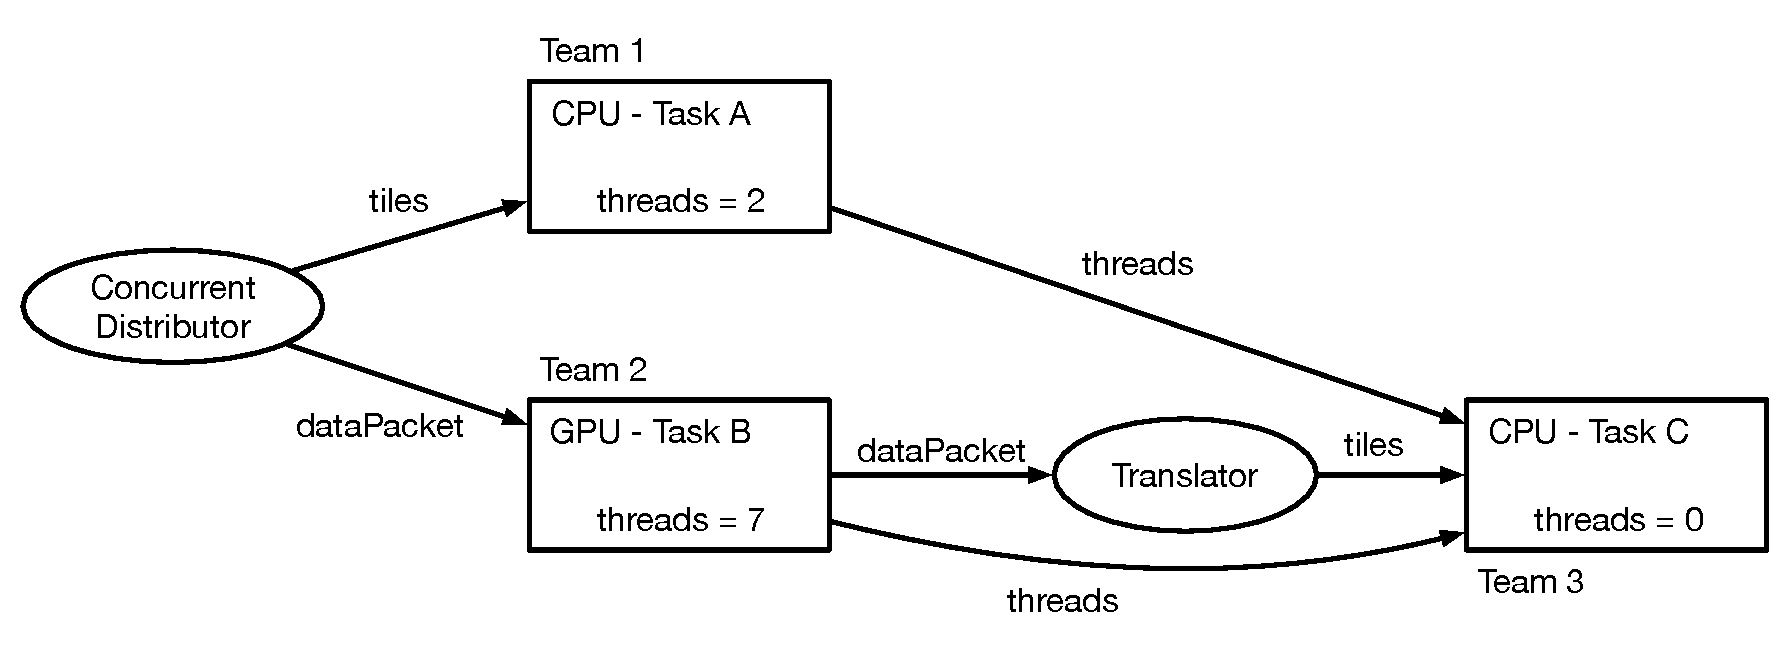
\includegraphics[width=5.5in]{ConcurrentItorExample.pdf}
\caption[]{An example of a runtime configuration of thread teams that implements
two concurrent pipelines using three thread teams.  We imagine that Task A and C
were written so that all code is run in the host and that Task B was written so
that it launches kernels on the GPU.  Therefore, the Task A pipeline runs
only on the host and is given only two threads to do this.  The Task B/C
pipline gives 7 threads to Team 2 so that it can flood the GPU as fast as possible with
kernels.  Once a data packet has had Task B applied to it on the GPU as
orchestrated by Team 2, the team moves the data back to the host, a work
translator enqueues the tiles in the data packet with Team 3, and Team 3 applies
Task C on a per-tile basis.  Note that there is little sense in giving Team 3
threads at the beginning as it needs units of work to first pass through Team 2.
Hence, it is given zero threads to start with.  However, as Teams 1 and 2 finish
their tasks, Team 3 will have threads activated and begin work.  It follows that
Team 3 could eventually have 9 activated threads applying Task C.}
\label{fig:ConcurrentItor}
\end{center}
\end{figure}

The second layer of parallelism exposed by the runtime design is that of forming
\textbf{task bundles}.  Specifically, the runtime interface has been designed so
that with each execution of the runtime, we can execute several work tasks with
certain pairwise dependence relationships.  For instance, if we bundle two tasks
that have no data dependencies at all, then these two tasks can be run
concurrently with one task run in the host and the other in a device.  In
addition, if we have a third task that has no dependence whatsoever with either
of the first two tasks or that must be run after the device task, then this
task may also be included in the bundle for running on the host after the device
task has been completed.  The two tasks in a task bundle that run concurrently
are called the \textbf{concurrent CPU} and \textbf{concurrent GPU tasks} if we are
running on nodes with host CPUs that offload to GPUs.  On a system with such nodes, a
task in the bundle that is run on blocks in the CPU memory after the concurrent
GPU task has been applied to these blocks is called a \textbf{post-GPU
task}.  Note that one can run the runtime with only one task in the bundle
if so desired.\\

This design therefore allows for parallelism in the form of task parallelism as
well as parallelism in the form of pipelining work on devices.  For instance, if a
runtime execution is scheduled with the GC fill asynchronous iterator, then the
stages in the pipeline are
\begin{enumerate}
\item{copy from the Grid unit's data structures in host memory to a host pinned memory
buffer those tiles with GC data already filled,}
\item{assemble $N$ tiles into a data packet and initiate asynchronous data
transfer to device,}
\item{launch in device all kernels that comprise the concurrent device task and
apply to all tiles in the data packet,}
\item{transfer asynchronously all tiles in data packet back to host memory
buffer,}
\item{copy all tile data in data packet back to Grid unit's data structures in
host memory, and}
\item{apply post-concurrency host task to all tiles in data packet.}
\end{enumerate}

In the concurrent CPU/GPU and post-GPU scenario we recognize that the runtime
effectively runs two pipelines concurrently and such that the post-GPU task is
an extension of the concurrent GPU task pipeline.  We understand, therefore,
that the runtime uses a single iterator over blocks to feed the two pipelines
and that each block is fed to both pipelines.  The code that iterates and feeds
blocks identically to all pipelines is a \textbf{concurrent work distributor}.\\

\begin{figure}[!ht]
\begin{center}
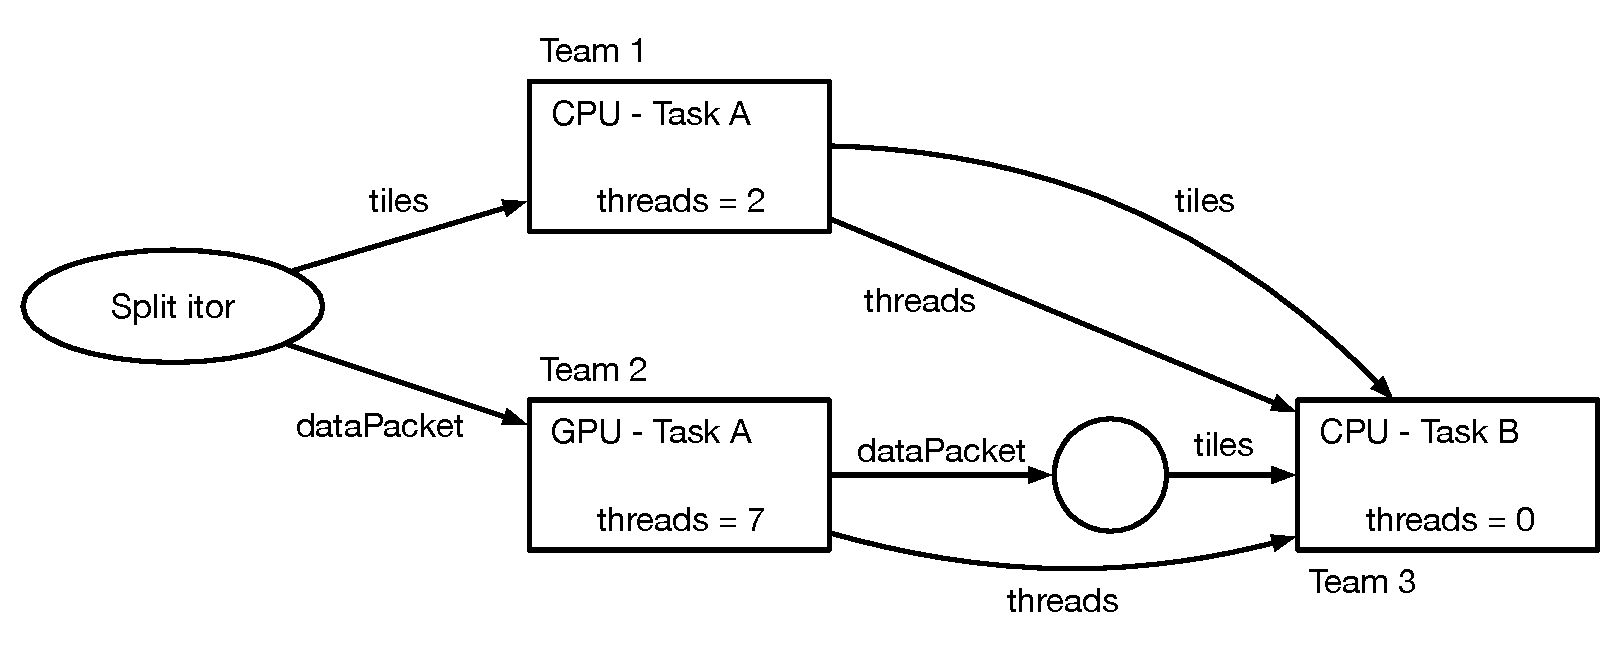
\includegraphics[width=5.5in]{WorkSplittingExample.pdf}
\caption[]{An example of a runtime configuration of thread teams that implements
a single, data-parallel pipeline.  We imagine that a host-only version of Task A
and a GPU version of Task A have been written so that the task bundle contains a
CPU Task A, a GPU task A, and Task B, which must be run after Task A.  The work
splitting distributor passes a fraction of the tiles to Team 1 and the
remaining tiles to Team 2 so that both host and GPU are used to apply Task A in
parallel.  Both of these teams are work publishers to Team 3 so
that this team can apply Task B to all tiles.}
\label{fig:SplitItor}
\end{center}
\end{figure}

The design of the runtime allows, however, for data parallel execution of a task
bundle.  For example, a CPU version and a GPU version of a single task could
be written by the offline toolchain and bundled together.  The single block
iterator in the runtime would then be instructed to partition the blocks so that
only a fraction of blocks are sent to the pipeline that runs the task on the
CPU and the remaining blocks sent to a second pipeline that runs the task on the
GPU.  In this case, the code that iterates over blocks and feeds the pipelines
is a \textbf{work splitting distributor}.\\

The concept of task is an element of a high-level software model.  The design of
the runtime includes a lower-level software model element, known as a
\textbf{thread team}, which are used to construct the aforementioned runtime
pipelines so that tasks can be mapped to node hardware and to allow for load
balancing of computing resources on the host, on which the thread teams run.
At startup, the runtime will create $N$ thread teams, each of which contains $M$
threads, where $N, M$ are setup-time parameters to be determined by the offline
toolchain.\\

Each thread team contains a single queue for holding pending \textbf{units of
work}, where units of work are either a tile or a \textbf{data packet} comprised
of one or more tiles.  While thread teams are not associated in any way with the
different devices in a node, it is understood that a thread team whose unit of
work is a tile will generally be used to apply its tasks to all given tiles
using the CPU.  Similarly, a thread team whose unit of work is a data packet
will generally be used to apply its task to all given tiles using an
accelerator with its own dedicated memory, which implies that the data packet
exists to manage the difficulties and time penalties associated with
transferring data between host and device memories.\\

For a single runtime execution cycle, each thread team to be used in the cycle
will be given exactly one task in the associated task bundle.  In addition, it
is instructed to activate a given number of its $M$ threads for applying its
task.  The activated threads are used to apply the single task to all units of
work given to the team during the execution cycle using dynamic scheduling.\\

In the task parallel example, we imagine that the concurrent CPU and post-GPU
tasks will be assigned to thread teams that work with tiles; the concurrent GPU
task, to a thread team that works with data packets.  The concurrent work
distributor will enqueue all tiles directly with the CPU task's team, aggregate
tiles into data packets, and enqueue a data packet with the concurrent GPU
task's team once each data packet contains enough tiles or there are no more
tiles left.  When the concurrent GPU's team has finished applying its task to
all tiles in a data packet, it gives ownership of the packet to a \textbf{work
translator} that will enqueue separately each tile in the data packet with the
team executing the post-GPU task.\\

A design element of the runtime that can enqueue units of work with a thread
team or a work translator is a \textbf{work publisher}.  The design elements
that receive the units of work in their queue are known as \textbf{work
subscribers}.  Similarly, thread teams can be configured as a \textbf{thread
publisher} and as a \textbf{thread subscriber}.  When a thread in a thread
publisher team determines that there is no more work to be done in the current
execution cycle and therefore deactivates, the thread informs the team's
subscriber that it can now activate another thread so that it can help the team
finished its task.  This allows for some control of the load balancing of the
threads running in the host.\\

The pipeline and thread team layout pertaining to the above task parallel
runtime example is shown in Figure~\ref{fig:ConcurrentItor}.  An example of a data parallel
runtime thread team configuration is shown in Figure~\ref{fig:SplitItor}.  Note that the
thread teams have been designed such that many different thread team
configurations can be built in to the runtime.  We hope that this aspect of the
design allows for easily scaling the runtime's capabilities as node architecture
grows in device diversity and in hardware complexity.  As the offline toolchain
determines how to bundle tasks, it is also hoped that having a large number of
such configurations will allow for effective bundling that leads to efficient,
parallel usage of all computational in-node resources.\\

\textcolor{red}{TODO: Where does the interface between the runtime and offline
tools lay?  Should the runtime be programmed with all possible thread team
configurations and expose these to the offline tools?  Or should the offline
tool determine which thread team configurations it needs and write the code
that assembles the teams into a configuration and executes a task bundle with
the configuration?}\\

A group of tasks are said to be \textbf{runtime-compatible} and can therefore be
bundled together into a single runtime execution if
\begin{itemize}
\item{they can be co-scheduled in the runtime such that they are executed in an
order that satisfies interdependencies and}
\item{the tasks are to be run on the same set of tiles or if one task is going
to iterator over tiles at a finer-grained structure and the second task can
complete its work on its set of tiles using the same structure.}
\end{itemize}
An example of the second case is if one task
will do its work by looping over all levels and iterating across all leaf blocks
at each level and the second task needs to do its work on all leaf blocks at all
levels.  Based on the discussion above, it is not necessarily the case that
runtime-compatible tasks can be run concurrently.  Also, the definition allows
for task bundles of auxiliary tasks (all tasks in the bundle iterate over the
empty set) and the runtime interface includes a routine for executing such a
bundle.\\

One can start to analyse the different data movements associated with particular
task bundles.  For instance, data that is operated on by a concurrent GPU work
task must obviously be transported back to the host memory in the case that a
post-concurrency CPU task is also included in the bundle and operates on or uses
the same data.  In the absence of this dependency, it is possible that the
concurrent GPU work task data could be left in the GPU's memory for immediate
use by following GPU-based tasks.  However, we cannot know that the device
memory will be large enough to contain this memory as well as memory needed by
the following GPU task.  Therefore, we must assume that all runtime executions
that contain a work task run on a device with its own physical memory have an
implied data transfer back to the host memory.\\

The current implementation of the \texttt{simpleUnsplit} Hydro code, while temporary and
brute force, contains an example of an implicit barrier that can exist between
consecutive tasks.  When tiling is not enabled, the solution at time step $n$ on
a given block can be used to compute fluxes and these used to overwrite in-place
the solution data with that of the $n+1$ time step on the same block.  In other
words, the compute flux and update solution tasks can be fused into one
computation to be done in one single iteration in a loop over blocks.\\

When tiling is enabled, however, the solution data cannot always be overwritten
in-place as this could update the data in interior cells that are in fact
guardcells of a different tile.  If this is done before the fluxes have been
computed in the neighboring tile, then the result will not be correct.
Therefore, in this case, the compute fluxes task must be run on all tiles and
saved in intermediate storage before the solutions are updated based on the
fluxes, which is an implied and required barrier that exists between
the two tasks and that prevents combining the two tasks into a single loop over
tiles.\\

% Consider the case of a loop over tiles that sets a value to a variable and
% where the value can only be determined after iterating over all tiles (i.e.
% something akin to a reduction).  If a second loop over the same tiles uses
% that variable, then an implied variable exists.

This example motivates the following statement.  Two or more tasks can be
\textbf{fused} if
\begin{enumerate}
\item{the tasks are to be run on the same set of tiles or if one task 
iterates over tiles at a finer-grained structure and the second task can
complete its work on its set of tiles using the same structure and}
\item{they have no data dependencies or appear in order in the task graph with
no implicit barrier between them.}
\end{enumerate}
This definition allows for fusing tasks from different operations and even from
different units.
Note, however, that it might be more advantageous in terms of decreased runtime
to avoid fusing so that the tasks can be run on different hardware.  Also,
fusion could lead to performance degradation if the register pressure is too
high for the fused task and frequent context switching is required by the data
access pattern.  \textcolor{red}{Two work tasks that are separated by
an auxiliary task cannot be fused without also fusing in the auxiliary task,
which could lead to either incorrect results or to unacceptable increases in
runtime.}\\

Note that runtime-compatible tasks that have no interdependence within a single
time step can be bundled together or run in different runtime executions freely
(\textit{e.g.} Gravity potential and hydro step) within their time step.  Also,
we can choose to fuse these two tasks in any desired order.  Runtime-compatible
tasks that have a dependence can be bundled together in the same runtime
execution if one is scheduled on the GPU and the other as the 
post-concurrency CPU task.\\

An potential side-effect of our design is that data movements (\textit{e.g.}
intranode, internode, or host-to-accelerator) that are required by an operation
will be expressed explicitly at the high-level representation of the operation.
In this sense, data movements will be placed at the same level of importance in
terms of algorithmic design as tasks.  Ideally, any two successive data
movements will be separated by only a single runtime execution.\\

Finally, we partition the code used at each time step into the three classes
\begin{enumerate}
\item{\texttt{Driver\_evolveFlash} and its auto-generated runtime calls,}
\item{\textbf{static Fortran routines} that carry out computations at the
level of a tile (\textit{e.g.} \texttt{hy\_computeFluxes}), and}
\item{the \textbf{patch panel} layer of code that must be auto-generated to
match the contents of \texttt{Driver\_evolveFlash} to the interfaces of the
static Fortran routines.}
\end{enumerate}
If a simulation is to be run in CPU-only mode, then the latter class of files
would consist of auto-generated high-level representations of each operation
(\textit{e.g.} Hydro.F90) that are functionally equivalent to the code presently
in FLASH5.  Otherwise these files would be auto-generated Fortran files that
implement each of the tasks being passed to a runtime execution.\\

\textcolor{red}{Do we need to classify intermediate data used by kernels?}

%%%%%----- ORCHESTRATION SYSTEM HIGH-LEVEL REQUIREMENTS -----%%%%%
\section{Overall System}
\subsection{Requirements}
Users shall be able to setup each simulation to run
\begin{enumerate}
\item{on CPU-only platforms with no runtime (\textit{i.e.} run in FLASH4 mode),}
\item{on CPU-only platforms but with a runtime so that independent tasks or
independent tasks/communications can be overlaid, or}
\item{on platforms that have host/accelerator heterogeneous node architecture.}
\end{enumerate}

We assume that FLASH5 will run on a variety of different machines including
personal laptops and leadership class machines.  The Orchestration System design
shall not expose to CPU-only/no-runtime users unnecessary configuration
complexity nor additional runtime penalties.  In particular, when run in
CPU-only mode, using FLASH5 shall be virtually identical to using FLASH4.\\

The system shall be comprised of
\begin{enumerate}
\item{an offline tool that constructs a decorated kernel control flow graph,}
\item{an offline tool that optimizes resource use and execution time by
determining how to order tasks, on which hardware to run each task, and
therefore how to form task bundles,}
\item{offline tools that generate simulation- and platform-specific Fortran code
based on the optimized scheduling of the previous tool, and}
\item{an orchestration runtime subsystem.}
\end{enumerate}
For more information regarding each of these subsystems, refer to its
associated, detailed design section below.\\

The kernel/task graph shall represent only the work that needs to be done at
each time step.  The information needed to construct the kernel/task graph shall
be made available at setup time so that the graph can be constructed offline at
setup time, which implies that the graph is static and valid for each
timestep.\\

The design shall allow for specification of runtime parameters that can alter
how the kernel/task graph is traversed at runtime.\\

The design shall allow for executing code between time steps, including
computationally-heavy code, that can make use of the orchestration runtime.
However, this code shall not require automatic optimization of scheduling nor
auto-generation of code and shall therefore not be included in the kernel/task
graph.  An example of such code is the regridding of the domain by an AMR-based
implementation of the Grid unit.\\

While it could be possible to run concurrently the final tasks from the $n^{th}$
time step with the beginning tasks for time step $n+1$, the orchestration
system shall not allow for such parallelism so that complexity is reduced.\\ 

The system shall be designed such that the bundling of tasks and relative
scheduling of these can be done as either a static task at setup time or at
runtime so that bundling and scheduling can be done dynamically in response to
acquiring actual runtime performance and resource usage data during a simulation
run.  \textcolor{red}{What does this mean in terms of configuration of this
subsystem?}\\

When the optimization of task/kernel scheduling is done at setup time, the 
code generation tool shall write at setup time Fortran code that will execute
all tasks with the same bundling and same relative ordering for each time
step.\\

When the optimization of task/kernel scheduling is done at runtime, the 
code generation tool shall write at setup time Fortran code that will allow a
forecasting scheduler to execute each time step with as many task bundles as it
sees fit.\\

Ideally, the public interface of the orchestration runtime shall not need to be
altered to accommodate running with static scheduling or runtime scheduling.\\

At each regridding, the Grid unit shall use the runtime to cache
non-tile-specific information in device memory.  Examples of such information
are
\begin{itemize}
\item{cell and face coordinates,}
\item{face areas, }
\item{cell volumes, and}
\item{[XYZ] mesh sizes.}
\end{itemize}
This information shall not change during the computations made at a single time
step so that available memory resources in different devices are fixed when the
time step starts.\\

\textcolor{red}{Should we insist that kernels also cache block-indexed values
like boundBox and physical size?  Do we get access to cached data through the
tileDesc object methods?  For example, when called on the host, the method
physicalSize will do the actual calculation.  However, when called on the GPU,
should the same routine just get the values from cache?}\\

Values that are needed in device memory for computation and that are constant
throughout the full program execution shall be stored in host memory and in all
device memory (where needed) at the beginning of program execution such that the
value is correctly mirrored across all memory systems and such that memory
usage can be correctly gauged by the runtime system at the start of each time
step.\\

Values that are needed in device memory for computation and that are constant
during a single time step shall stored in host memory and in all device memory
(where needed) at the beginning of the time step such that the value is
correctly mirrored across all memory systems and such that memory usage can be
correctly gauged by the runtime system at the start of each time step.

%%%%%----- STATIC FORTRAN CODEBASE -----%%%%%
\section{Static Fortran computational code}
\subsection{Requirements}
The routines defined in the static Fortran computational code shall each operate
on a single tile or on no tile at all.\\

The routines defined in the static Fortran computational code shall not
dynamically allocate memory.  Rather, the necessary tiles of memory shall be
passed in from the highest-level of such routines.  In other words, all memory
management is done at the level of each operation and the tiles of scratch
memory needed by each static routine and all its subroutines must be passed into
the static routine and passed through the interface to the subroutines.

\subsection{Possible Requirements}
The static Fortran routines shall not be exposed to the notion of a tile and
therefore shall not contain the Grid unit's tile descriptor as a parameter.
Rather, all tile-specific information shall be obtained from the Grid unit by
the operation at the highest level and all such information passed to static
Fortran routines as individual parameters.  This shall be implemented so that
Grid information cached in device memory can be used immediately within device
kernels.  \textcolor{red}{This means that the high-level routines will have very
long parameter lists.  Does passing in so many parameters have an adverse effect
on memory or performance?  Larger frame sizes?}

%%%%%----- ORCHESTRATION OFFLINE TOOLCHAIN -----%%%%%
\section{Composer design}
%The composer should have four levels of hierarchy, with each hierarchy
%having its own set of meta information encodings. The meta information
%encoded should be such that the composer tool can infer dependencies
%easily. 

\subsection{Simulation Unit Level Metadata}
\begin{itemize}
\item Any customization at Kernel, Task or Operation level, which also
  tells the tool which composer metafiles to ignore in the source tree
\item Recipes for combining operations -- perhaps we one can even build a
  database of recipes for combining operations similar to shortcuts
\item Recipes for allocating work to communicators/devices
\end{itemize}
The composer tool will start from the simulation unit, just as setup
tool does. It will assemble all the metadata files it needs to parse,
and as a first step replace all the default ones with custom ones
included in the Simulation unit. It will then start to build up the
information from bottom level up. If the simulation unit is asking to
replace a recipe at any level, the tool will check it for feasibility
and abort if it isn't. This might be quite difficult, we will have to
think about it more. 
 
\subsection{Kernel Level Metadata}
\begin{itemize}
\item State variables operated on
\item State variable modified
\item Spatial dependences (pointwise or not)
\item Temporal dependences (uses items computed in previous
  iteration)
\item Dimensionality
\item Branches in the kernel -- are they before, in the middle of, or
  at the end of the kernel
\item Keyword $\implies$ code dictionary if applicable
\item Whether a compute intensive kernel
\item scratch space needed
\end{itemize}
After parsing all the information the composer tool will know the
complete set of state variables that may be used and modified in the
task, and what kind of spatial and temporal dependencies exist in
whole of the task. The advantage will be if there are none, that
information can be percolated up all the way to the operation level composer.

\subsection{Task Level Metadata}
\begin{itemize}
\item The number of kernels in the task
\item Mutually exclusive kernels (branching at the kernel level)
\item Where can scratch asked by kernels can be reused within tasks
\item Critical path of kernels -- optional 
\item Recipes for composing kernels -- optional
\end{itemize}
At this level the composer tool is still tracking spatial and temporal
dependences, and from doing some branch analysis can tell the
reusability of data between kernels, especially if recipes are
provided. 

\subsection{Operation Level Metadata}
\begin{itemize}
\item The number of tasks
\item Recipes for composing tasks
\item Communications between tasks
\item Reductions, and the state modified with reductions
\item Tasks available for interleaving with other operations 
\item Operations it can overlap with
\end{itemize}
At this level the composer knows whether it can compress data to be
sent to devices in terms of number of ghost cells, and consolidated
memory mapping needs of the operation.

\subsection{Example}
Unsplit Hydro time step operation
\begin {itemize}
\item At kernel level all hy\_uhd.... functions, some may be split
  further.  No temporal dependencies within kernels, spatial dependency
  is defined by the stencil. Branches mostly at the beginning or at
  the end of each kernel. 
\item Most variables used and updated, should be enumerated
\item At task level one can convert all of Dongwook's case statements
  into recipes. 
\item At the operation level recipes are one of three ways of using flux
  correction. Some recipes may involve interspersed gravity
  calculation
\item The operation will clearly state that it cannot overlap with any
  other physics unit in the same timestep calculation.
\end{itemize}
Gravity with multipole implementation
\begin{itemize}
\item All grav\_... functions are kernels.
\item The number of tasks is two. The computation of moments has no
  spatial or temporal dependency (I think). 
\item In first task density is used, nothing is modified, in the
  second task potential is modified, nothing is used.
\item Reduction in between the two tasks is indicated
\item Tasks can be overlapped, as can be the reduction
\end{itemize}
Burn
\begin{itemize}
\item No kernel has temporal or spatial dependency
\item Species and density used and modified.
\item One task, can be overlapped
\end{itemize}

Now if we were putting together a Sedov application there would be no
specific information needed at the simulation level, and no
recipes. If we were doing a supernova calculation then we would
provide a recipe for overlap of burn with gravity.

\subsection{Requirements}

The macros used to index different variables in FAB data storage shall be
constructed so that macros with different names never refer to the same
variable (\textit{i.e.} we prevent aliasing any region of data) so that
read-write dependencies of data can be established conservatively and correctly
without having knowledge of the macro mapping to indices\footnote{I do not
believe that the Unsplit implementation of the Hydro unit presently satisfies
this rule}.\\

The offline tool that constructs the kernel/task graph shall determine
automatically for each kernel
\begin{itemize}
\item{which data variables (\textit{e.g.} UNK, face-centered, fluxes,
\textit{etc.}) are read,}
\item{which data variables (\textit{e.g.} UNK, face-centered, fluxes,
\textit{etc.}) are written,}
\item{if the kernel is pointwise or stencil-based, and}
\item{the temporal dependence of the kernel computation.}
\end{itemize}

Rules shall be created that allow for determining task- and operation-level
metainformation based solely on the metainformation of all kernels used by the
task or operation.  \textcolor{red}{Say this with specific detail and
potentially just write the rules.}\\

Each work task should be labeled by the type of tiles on which it should be
applied (\textit{e.g.} leaf), to which level the tiles are restricted (if any),
and if the tiles are tiles or actually blocks.  This information is needed to
determine which iterator to use and to help determine which tasks are
runtime-compatible.\\

If a runtime execution if preceded by a data movement that can make use of an
asynchronous task iterator, then the offline tool shall build the runtime
execution such that the execution uses the asynchronous task iterator
internally.  Note that it is exactly this possibility that motivates the
possible need for multiple data packets per task.

\subsection{Possible Requirements}

%We prefer static analysis of static Fortran routines to determine dependencies
%between tasks as opposed to writing directives to express this.  If we do a
%static analysis within the scope of the single file, then we do not know that
%the variables with different names are actually different (unless we go outside
%the file and look at Flash.h).  Going outside the file is too complex.  We could
%agree on a rule (like restrict in C++), where we say that all MACROS that end
%with \_VAR and that are used with a four-dimensional array and are different if
%the part preceding \_VAR are different.  The third option is explicit decoration
%like Anshu has, which increases the likelihood of errors.  Note that unsplit
%does not presently allow for us to make strong statements about the MACROS as
%they have two sets that have the same mapping but two names (DENS\_VAR and
%DENS\_01\_VAR).\\

%Should we allow for fusing of two tasks that are completely unrelated
%(\textit{e.g.} from different operations and possibly units)?  This could be
%good if we have two computations that are individually too light weight to
%justify the data transfer to the GPU but together form a computationally-heavy
%load.  Note that fusing could be a bad idea if the register pressure grows too
%strongly due to the fusion.\\

%However, it
%might be more advantageous in terms of decreased runtime to avoid fusing so that
%the tasks can be run on different hardware.  The developer shall be able to
%specify default information to help determine if tasks should be fused and on
%which type of device to run in the case that the tasks are not fused.  The users
%shall be able to override the default values set by the developer to help
%influence fusing and on which non-fused tasks should be run.  Two
%runtime-compatible tasks cannot be fused if there is a barrier between them.
%For example, the stencil nature of \texttt{simpleUnsplit} means that if we use tiling,
%then there is am implied barrier between computeFluxes and updateSoln.  However,
%if tiling is turned off, then the barrier is not implied and we can fuse.
%\textcolor{red}{How to determine this and/or encode it?}\\

%\textcolor{red}{What is the criterion for distinguishing between a task and a
%kernel?  For instance, we could say that energyFix and Eos are kernels within a
%task or say that these are different tasks and they inherit their iterator info
%from the enclosing updateSoln.  Some of this is encapsulation/design.  We would
%like updateSoln to finish only once *all* the data is in its final, clean form.}

%%%%%----- OFFLINE CODE GENERATION -----%%%%%
\section{Offline code generation tool}
\subsection{Requirements}
If a simulation is setup such that no runtime is needed, then the offline tools
shall use the kernel/task graph to write a Fortran file that implements the
highest-level flow of each operation including looping over tiles, executing
data movements, and executing computation with calls to the static Fortran
computational code.  The resultant code shall be functionally equivalent and
similar in resource usage and runtime to the current Fortran code in FLASH4
(\textit{e.g.} \texttt{Hydro.F90}) except for the possibility that the generated
code might not contain mutually-exclusive branch statements (\textit{e.g.} use
LLF or HLL version of the simpleUnsplit solver).\\

If a simulation is setup to use the runtime with static scheduling, then the
offline tools shall use the kernel/task graph to run task bundles \textit{via}
the orchestration runtime by writing these to \texttt{Driver\_evolveFlash}.

If a simulation is setup to use the runtime with dynamic, forecasted scheduling,
then the offline tools shall auto-generate a layer of static code that will
allow for runtime execution of an unknown number dynamically-bundled
tasks at each time step and such that tasks are still executed in correct order.

\subsection{Possible Requirements}

%%%%%----- ORCHESTRATION RUNTIME DESIGN SECTION -----%%%%%
\section{Runtime design}
\label{sec:Runtime}

\textcolor{red}{TODO: Need to add in brief explanation of thread teams,
execution cycles, and topologies of thread teams.  This document should
eventually end up in the Orchestration System design document, in which case
this information could go in the executive summary.}\\

\textcolor{red}{What classes of scalar values do we have in the physics units?
For instance are there scalars that are constant for the duration of the
simulation?  Constant for the duration of an iteration?  Constants that are
changed by auxiliary tasks?  Constants that are updated by work tasks?  For the
first two, we can set up mirrors of the variable between host and devices.
Those that are changed by auxiliary tasks can also be mirrored by running the
task concurrently in both the CPU and the GPU.  What about the others?  Do we
send those in the data packets so that the CPU and GPUs can force the mirroring
somehow?  Do we just hand these over to managed memory and hope that everything
goes well?  Do we hand these over to managed memory but ask the offline
toolchain to touch the scalars on the appropriate device before each runtime
call (these are blocking)?}

%The class implements a team of threads that is specifically designed for use
%by the Orchestration Runtime, which schedules a single task with the thread
%team for execution in a single cycle.  All public methods are thread-safe.
%
%The team is designed and implemented as an extended finite state machine
%(EFSM).  The mode (qualitative) portion of the EFSM's state must be in one
%and only one of
%  - Idle,
%  - Running with the work queue open
%    (i.e. able to accept more units of work),
%  - Running with the work queue closed
%    (i.e. no more units of work can be added),
%  - Running with no more pending work
%    (i.e. there are no more units of work in the queue, but at least one
%    thread is still applying the task to a unit of work), or
%  - Terminating   
%at any point in time.  The internal state variables (quantitative) for the
%EFSM are the number of
%  - pending units of work in the team's queue,
%  - Idle threads,
%  - Waiting threads,
%  - Computing threads, and 
%  - Terminating threads.
%The events that trigger state transitions are
%  - an external call to startTask()
%    (Idle -> Running \& Open),
%  - an external call to closeTask()
%    (Running \& Open -> Running Closed),
%  - a thread determines that the queue is empty
%    (Running \& Closed -> Running \& No Pending Work),
%  - all threads have transitioned to Idle
%    (Running \& No Pending Work -> Idle), and
%  - an external call results in the destruction of the thread team object
%    (Idle -> Terminating).
%At construction, the thread team starts the maximum number of threads
%allotted to it and these persist until the team is destroyed.  The EFSM
%starts in the Idle mode with all threads in the Idle state and an empty
%queue.
%
%External code starts an execution cycle by calling startTask and at the same
%time indicates what task is to be executed by the team as well as how many
%threads in the team shall be activated immediately to start applying the
%task.  After startTask has been called, external code can use the enqueue
%method to give to the team tiles on which to apply its task.  These tiles are
%passed to enqueue one unit of work at a time where a unit of work could be a
%single tile (e.g. if the task will have the team run computations on a CPU)
%or a data packet containing multiple tiles (e.g. if the task will have the
%team run computations on an accelerator).  The external code indicates to the
%EFSM that all tiles on which to operate during this cycle have already been
%enqueued.  The EFSM then continues its application of the task to all
%remaining given tiles and automatically transitions back to Idle once work
%and, therefore, the execution cycle finishes.  An external thread can be
%blocked until the task execution cycle finishes by calling the team's wait
%method.
%
%There is no restriction that a single thread team must execute the same task
%with every execution cycle.  Similarly, there is no restriction that a team
%must be dedicated to running computation-heavy code on only a single piece of
%hardware (e.g. only on the CPU or only on the GPU).  Rather, the thread team
%only knows to execute the code behind a function pointer, which can include
%kernel launches on an accelerator.  It is possible for that code to execute
%computationally-heavy code on a mixture of available HW on the node.
%However, our present best guess is that restricting each task to run
%principally on a single device is likely clean, simple, elegant, and
%maintainable.
%
%The EFSM is implemented using the State design pattern presented in the Gang
%of Four's famous Design Patterns book (Pp. 305).  This class exposes the
%interface of the EFSM to client code and the client code should only
%instantiate this class.  Each of the ThreadTeam* classes derived from
%ThreadTeamState are instantiated once by this class and are used to provide
%state-specific behavior of the team.  This design was chosen as the response
%to events, outputs, and error checking of the EFSM are logically partitioned
%across the modes of the EFSM and are therefore largely encapsulated within
%each class.  This class
%  - declares and houses all data members needed to implement the EFSM,
%  - initializes the EFSM in the correct Idle state,
%  - handles the destruction of the EFSM, and
%  - defines how all threads in the team shall behave.
%Note that each thread in the team is a FSM that moves between the Idle,
%Waiting, Computing, and Terminating states.  The hope is that studying,
%analysing, and maintaining the EFSM will hopefully be easier thanks to the
%use of this design.  However, the runtime efficiency of this design has not
%yet been studied.
%
%It is envisioned that the runtime may instantiate multiple thread teams with
%each team executing a potentially different task.  See the OrchestrationRuntime
%documentation for more information regarding this intent.
%
%To control the number of active threads running in the host at any point in
%time, a thread team can become a thread subscriber of another thread team so
%that the subscriber is notified that it can add another thread to its team
%each time a thread terminates in the publisher thread's team.
%
%To control the number of active threads running in the host at any point in
%time, a thread team can become a thread subscriber of another thread team so
%that the subscriber is notified that it can add another thread to its team
%each time a thread terminates in the publisher thread's team.
%
%In addition a thread team can also be setup as a work subscriber of another
%thread team so that when the publishing thread finishes a unit of work, the
%result is automatically enqueued on the subscriber team's queue.  When the
%publisher has finished all its work and enqueued all work units in the
%subscriber team, the publisher automatically calls the subscriber's closeTask
%method.
%
%Note that a thread publisher can only have one thread subscriber and a work
%publisher can only have one work subscriber.  However, a thread team can be
%both a thread subscriber and a thread publisher.  Also, a thread team can be
%a thread subscriber for one team and a work subscriber for another.
%
%The implementations of the publisher/subscriber design aspects are
%one-directional versions of the Observer design pattern (Pp. 293).
%
%The wait() method for a publisher team must be called before the wait()
%method of its subscriber team.

%%%%%----- RUNTIME REQUIREMENTS SUBSECTION
\subsection{Runtime Requirements}
The statements made in this section are intended to be informal, high-level
requirements.  Specifically, they should be correct for all orchestration
runtime designs and ideally require little change if our design changes
significantly.  In other words, these statements should not be informed by
implementation ideas or details.

\begin{req}
\textcolor{red}{We should be able to send tiles to CPUs but build data packets
of blocks.}
\end{req}

\begin{req}
The runtime implementation and dependencies shall not impede FLASH5 from being
used on *nix operation systems including macOS nor from being run for research
on laptops.  Implementations shall not require more than the C++-11 standard and
threading implementations shall be portable.  \textcolor{red}{What Fortran
standard are we shooting for?  If the runtime is written in C++, then we will
need F2003 for the code that manages the C++/Fortran interoperability.  Ideally,
we can get rid of classes and restrict all other Fortran code to F95.}
\end{req}

\textcolor{red}{Present implementation is with pthreads, which is portable based
on OS (is it compliant with the POSIX standard).  If we do accept the C++-11
standard as reasonable, then the runtime implementation could be redone to use
the C++ thread facilities.}\\

\textcolor{red}{Memory managers such as AML and Umpire are dependent on
LibNuma, which is linux based.  Therefore, macOS users would presently not be
able to use a runtime based on these.  For laptops, this might be acceptable.
However, this would preclude Mac Pro users from using their GPUs.}

\begin{req}
If a simulation is setup such that no runtime is needed, then the Orchestration
runtime shall not be built into the simulation.  In particular, this means that
there shall be no unnecessary resources allocated nor an extra level of packing
tiles into data packets.  This could allow for basic stub implementations such
as initialization/finalization being called from Driver.
\end{req}

\begin{req}
At any point in time during the execution of a simulation, there shall be no more
than one instance of the runtime in operation so that design complexity can
be minimized (\textit{e.g.} resource allocation and management).
\end{req}

\begin{req}
\label{req:UnitImplementations}
The runtime shall be built into FLASH5 as a new unit and the unit shall allow
for different implementations of the unit.  Some examples of different
implementations will be
\begin{itemize}
\item{low-level (\textit{e.g.} CUDA) \textit{vs.} high-level
(\textit{e.g.} OpenMP) and}
\item{general (\textit{e.g.} CUDA) \textit{vs.}} platform-specific
(\textit{e.g.} CUDA optimized for Summit).
\end{itemize}
\end{req}

\begin{req}
All implementations shall be designed for portability.  As an example,
\textit{general} use GPU-related code shall avoid using device-specific library
functionality such as managed memory as other GPU-based platforms might not
offer managed memory at all or in a portable way.
\end{req}

Clearly the above requirement is ill-defined and therefore decisions regarding
what does and doesn't satisfy the requirement will involve personal judgement
and trade-off analysis.  For example, emphasis was placed on the word
``general'' above as Req~\ref{req:UnitImplementations} would allow for a
CUDA-based implementation that uses managed memory.  However, if we choose to
have two different implementations of large, complex, general-use code that is
hard to test such that the two implementations differ only in a few lines
related to mananged memory, then we might decide that maintainability is being
significantly decreased.

\begin{req}
The interface of the runtime shall be designed such  that when a new type of
device is introduced in platform nodes, the routines for starting a runtime
execution cycle can be extended trivially\footnote{Ideally by adding new function
pointers to the parameter list of these routines.} for including the running of
tasks on these devices.  If the nodes allow for running concurrently tasks on
this device while running code on the host or on other devices, then the updated
interface shall allow for this.
\end{req}

\textcolor{red}{Where does the interface between the offline toolchain and
runtime sit?  Should the runtime dictate what thread team topologies are
available and therefore fix the number of thread teams available and how the
toolchain maps work onto teams/HW?  Or should the offline toolchain write the
code that creates the topologies and therefore customize the runtime's interface
for launching execution cycles?}\\

\textcolor{red}{Put in information regarding runtime parameters needed by
runtime.  Does this include runtime parameters that depend upon how task were
bundled/scheduled?  If we have a parameter that specifies how many blocks to
include in the first data packet, then we should allow for a value that
specifies that all blocks should be included.  This might be useful for some
kernels that don't use the asynchronous iterator.}\\

\textcolor{red}{Do we allow for specifying to the runtime which data should
remain where?}

\begin{req}
At instantiation, the runtime shall instantiate a given number, $N$, of distinct
thread teams and each thread team shall be allowed to simultaneously use
at most a given number, $M$, of threads.  \textcolor{red}{It remains to be seen
if the threads should be created at instantiation and persist throughout the
simulation or if they should be created each time the runtime executes a task
bundle.  The former would be more runtime efficient, but permanently consume
more memory in the form of thread stacks, etc. and increase the burden on the
OS.  Is $M$ fixed across all thread teams?  TODO: Time thread team creation and
a no-op execution cycle to get an idea of orders of magnitude.  Determine size
of thread team in memory and size of thread footprint.}
\end{req}

Note that it is the client code's responsibility to determine $M$ and $N$ in
accord with the runtime requirements and technical specifications presented
here.

\begin{req}
Each thread team shall
\begin{enumerate}
\item{be created and run in the host CPU,}
\item{be associated with a single MPI rank,}
\item{be associated with a single unit of work (\textit{e.g.} tiles, blocks, or a
data packet of blocks), and}
\item{expose the same interface to client code regardless of the unit of work.}
\end{enumerate}
\end{req}

\begin{req}
For each execution cycle, a thread team shall be used by client code to apply at
most one task (work or auxiliary) to a subset of the tiles managed by the team's
associated MPI rank.  For the case of an auxiliary task, the subset is the empty
set.  The restriction to one task will help make it easier to determine
independence of tasks and teams.  For each cycle, the client code shall inform
the thread team what task shall be executed and how many threads in the team
should be activated immediately to start work on the task.  This implies that
the task assigned to a particular thread team can change from one execution
cycle to the next.
\end{req}

\begin{req}
All thread team units of work shall encapsulate each tile in the unit of work
with metainformation so that tasks can retrieve information such as coordinates
as well as the pointer to the location of the tile's data in relevant memory
systems.  If a task will only run on the host, then the unit work only need
identify the location of the tile's data (cell-centered, face-centered,
\textit{etc.}) in the host memory (i.e. the Grid unit's data structures).  If
the task will run in both CPU and in accelerators, then the metainformation must
specify pointers for all data in the memory accessible to the host and
accelerators.  \textcolor{red}{This requirement will need improvement as the
prototype evolves.  Basically, we are extending the notion of tile metadata to
the notion of a data packet.}
\end{req}

\begin{req}
Thread teams shall not need to know nor be informed of which device will carry
out the computation associated with a given computational task.  Rather the
given computational task shall know where its block data resides in different
memory and the task shall be written so that it can carry out its computations
on the devices assigned to it.  This can include running code on the host CPU
with the given team thread or using the team thread to launch computations on
accelerator devices.  \textcolor{red}{This requirement is also related to data
packets and will need improvement as the prototype evolves.}
\end{req}

\begin{req}
Each task to be run with a thread team shall have the same identical code
interface so that task-specific information does not need to be passed to the
task by the thread team.  This requirement helps decouple the thread team and
therefore the runtime from the work being done by the thread teams.
\end{req}

This implies that client code must devise a scheme that makes all
task-/computation-specific parameters available to the function that defines the
task.  For FLASH, our present design is to implement all task functions as
routines in a unit and all such parameters as data members in the unit.  This
means that the code that calls the runtime will need to set the values of these
data members before the call.  \textcolor{red}{For C++, would this mean wrapping
each task or a set of related tasks in a class?  Could we just package up
related parameters in a single namespace so that they are global but in an
acceptable way?}


\begin{req}
The thread team interface shall allow for client code to assign units of
work to a thread team one unit at a time where the full work load given to a
team during a single task execution is a subset of the blocks managed by the
team's associated MPI rank.
\end{req}

\begin{req}
The thread team interface shall allow for client code to inform the team when
all units of work to which the current task are to be applied have been given to
the team.  This shall include the possibility of giving a thread team a task but
no units of work.
\end{req}

\begin{req}
Client code shall trigger \textit{via} the runtime interface a single runtime
execution cycle that consists of executing potentially many distinct tasks (both
auxiliary and work) on multiple different target devices.  The runtime interface
shall provide the client code with a means to express what tasks are to be run
as well as inter-task dependencies such that the runtime will be able to
assemble an appropriate topology of thread teams that does not violate the
inter-task dependencies.  The runtime shall throw an error if the number of
tasks in the bundle is more than the number of thread teams created by the
runtime.
\end{req}

\textcolor{red}{What does this look like?  The offline toolchain should
determine the inter-task dependencies, the mapping of tasks to HW, and the
mapping of tasks to thread teams.  Is the latter just choosing a thread team
with the correct unit of work?  How does the toolchain specify to the runtime
which topology to use and the mapping of task to teams in the topology?  Can it
just be a long parameter list with multiple consecutive parameters in the list
specifying the task for a particular device?  The runtime could then see which
parameters specify a task and infer the topology from this.  We would need, for
instance, a CPU concurrent task, a GPU concurrent task, and a post-GPU task.}

\begin{req}
The runtime shall contain a \textbf{concurrent work distributor} that
facilitates applying multiple distinct tasks to all the blocks managed by the
runtime's MPI rank.  Specifically, this distributor shall gather tiles using the
Grid unit's tile iterator (or asycnrhonous tile iterator), form these into the
appropriate units of work, and give the units of work to the appropriate thread
teams.  Refer to Figure~\ref{fig:ConcurrentItor} for an example of such a scheme.
\end{req}

\begin{req}
The runtime shall contain a \textbf{work splitting distributor} that facilitates
using more than one thread team to apply a single task to all the
blocks managed by the runtime's MPI rank where the task is applied to
each block by one and only one team.  Specifically, this distributor shall
gather tiles using the Grid unit's tile iterator (or asycnrhonous tile
iterator), use a distribution scheme to determine which tiles will be sent to
which team, form these into the appropriate units of work based on the
destination team, and send the units of work to the appropriate thread teams.
Refer to Figure~\ref{fig:SplitItor} for an example of such a scheme.
\textcolor{red}{Allow for scheme that selects routing of work to team
dynamically?}
\end{req}

\begin{req}
A thread team may be configured to push units of work, to which it has already
applied its task, to another thread team.  The team that pushes units of work is
therefore a \textbf{work publisher} and a team to which units of work are
pushed is a \textbf{work subscriber}.  It shall be possible for a single thread
team to be a work subscriber for any number of distinct work
publishers\footnote{Split the load of blocks between a thread team dedicated for
FPGAs and a second team for GPUs.  We could have each team run the same task on
its subset of blocks and then pipe the results into a single work subscriber
that runs a quick, independent follow-up task on the CPU.}.  Note that work
distributors are therefore work publishers and that a single thread team may be
both a work subscriber and work publisher.  \textcolor{red}{The concurrent work
distributor is an example of a publisher that pushes units of work to multiple
subscribers.  Should this be allowed generally?  Use case would be using a
single thread team to apply a single task that must be done first and then
passing data to two teams that concurrently apply independent tasks.}
\end{req}

\textcolor{red}{The present implementation does not yet support multiple work
publishers for a single subscriber.  The design needs to be extended so that
a subscriber with multiple publishers can keep track of which publisher has
called closeTask.  The transition to Running \& Closed Queue would only occur
once each publisher has called closeTask.  Do we need a pub/sub pattern with
two-way knowledge?}

\begin{req}
\label{req:ThreadSubPub}
Each thread team may be configured as a \textbf{thread publisher} and as a
\textbf{thread subscriber}.  A thread publisher shall have at most one thread
subscriber and there shall be no limit to the number of thread publishers that a
thread subscriber can have.  When a thread in a thread publisher team determines
that there is no more work to be done in the current execution cycle and
therefore transitions to Idle, the thread publisher shall inform its
single\footnote{This requirement is related to load balancing and in this sense,
we cannot activate a thread in each of several thread teams because one thread
in the publisher team has transitioned to Idle.  We could build in a round-robin communication
scheme but choose not to in the name of simplicity.} subscriber that the
subscriber can now activate another thread in its team.
\end{req}

\begin{req}
A thread team shall not be allowed to push a thread or work to itself.  However,
the runtime shall not be responsible for ensuring that a given configuration of
thread teams does not lead to an endless cycle of feeding threads around a
circle of teams nor an endless cycle of feeding work around a circle of teams.
\end{req}

\begin{req}
\label{req:ThreadBalance}
If a thread subscriber is informed that it may activate another thread in its
team but there are no more Idle threads in the team, then the subscriber team
shall emit an error.
\end{req}

This implies that it is the client code's responsibility to ensure that the
number of threads in a thread subscriber team is less than or equal to the sum
total of threads that the team starts with and the number of threads that can be
activated.  Note that multiple thread teams can be connected in chains and a
single thread team could be a subscriber to many chains.  Therefore, the task of
determining the maximum number of threads in a thread subscriber team is important.

\begin{req}
The runtime shall allow for a thread team whose unit of work is a data packet of
blocks to be a work publisher for a thread team whose unit of work is a data
packet of blocks or whose unit of work is tiles.  Motivated by the latter case,
the runtime shall provide an object that breaks data packets of blocks into its
constituent tiles and enqueues these individually with a thread team.  For this
case, this object is the work subscriber of the first team and the work
publisher of the second team.  See Figures~\ref{fig:ConcurrentItor}
and~\ref{fig:SplitItor}.
\end{req}

\textcolor{red}{Is there a use case having a tile-to-data packet aggregation
object?}

\begin{req}
The runtime shall have a record/replay facility so that thread teams can be
arranged into a pre-described topology and each thread team setup in a given
state.  This should be useful for both debugging and designing meaningful direct
tests of low-level functionality.
\end{req}

%%%%%----- RUNTIME TECHNICAL SPECIFICATIONS & DESIGN SUBSECTION
\subsection{Runtime Technical Specifications \& Design}
The statements that appear in this section are being referred to as technical
specifications rather than requirements in that these statements are low-level
and directly informed by the design and how we plan to implement the design.
Therefore, it is expected that a change in the design that does not violate the
above requirements could still require significant changes to the technical
specifications in this section.\\

One main intent of the technical specifications is to highlight \textit{some} of
the key ideas, difficulties, complexities, and subtleties that should be kept in
mind when studying and maintaining the code.  Also, use, corner, and edge cases
that have been identified are presented as motivation for technical
specifications.  Finally, some statements are made because the correctness of
the design and implementation require that they be satisfied.  For such
statements, proofs are given to explain how we know that the specification is
satisfied by the design and actual implemetation.

%%-- THREAD TEAMS SUBSECTION
\subsubsection{Thread Teams}
A thread team is fundamentally event-driven software and as such its design has
been specified as a finite state machine (FSM).  However, the behavior in a
given state cannot be specified solely by a single qualitative state variable.
Rather, the behavior will depend on a qualitative state variable, which is
called the mode, as well as the quantitative internal state variables $N_i, N_w,
N_c, N_Q$ that respectively keep track of 
\begin{itemize}
\item{the number of Idle threads in the team,}
\item{the number of threads that are Waiting for work to be added,}
\item{the number of threads applying a task on a unit of work, and}
\item{the number of units of work in the team's pending work queue.}
\end{itemize}
Note that the definitions of $N_i, N_w, N_c$ imply that each thread is
always in one and only one of the Idle, Waiting, and Computing states but that
this EFSM need not track the actual state of each thread --- it is only the
aggregated thread state information that is important.  Therefore, the runtime
is an extended finite state machine (EFSM)
\[
M = (Q, X, I, O, s_0, T)
\]
where
\begin{itemize}
\item{$Q$ is the finite set of qualitative modes,}
\item{$X = \set{(N_i, N_w, N_c, N_Q) \in \Z_{\ge 0}^4\,|\,N_i + N_w + N_c =
N_{max}}$ is the set of internal state variables where $N_{max}$ is the
number of threads in the team,}
\item{$I$ is the set of internal and external events,}
\item{$O$ is the set of outputs,}
\item{$s_0 = (q_0, x_0) \in Q \times X$ is the initial state, and}
\item{$T : Q \times X \times I \to Q \times X \times O$ is the transition
function that is evaluated by the EFSM at each occurrence of an event to
identify the output to be performed as well as the state to which the EFSM must
be transitioned.}
\end{itemize}

Note that the set of all possible states is not $Q \times X$.  There are
elements in that set that the EFSM must not occupy.  See
Specs~\ref{spec:Closed_NoWork} and~\ref{spec:NoMoreWork_NeedThread} for examples
of such prohibited states.  Therefore, the above specification of $T$ is only
correct if we assume that the output associated with such prohibited states is
to inform client code of an error so that the EFSM can be terminated.\\

The set $Q$ contains the modes
\begin{itemize}
\item{\TeamIdle --- all threads Idle and no work in the queue}
\item{\TeamRunningOpen --- a task has been given to the team and units of work
on which to apply the task can still be given to the team (\textit{i.e.} an
execution cycle has been started)}
\item{\TeamRunningClosed --- a task is being applied but no more units
of work can be given to the team in the current execution cycle}
\item{\TeamRunningNoMoreWork --- a task is being applied, no more
units of work can be given, and the team has identified that the task has
already been applied to or is currently being applied to all units of work given
to the team for the current execution cycle}
%\item{\TeamTerminating --- the client has indicated that it no longer needs the team.}
\end{itemize}

The set $I$ of events is the union of events triggered by clients through the
team's interface
\begin{itemize}
\item{\texttt{startTask} --- give the team a task and activate a given number of the
$N_{max}$ Idle threads in the team to work on it}
\item{\texttt{increaseThreadCount} --- activate a given number of Idle threads in the
team so that they can start working on the task as well}
\item{\texttt{enqueue} --- give the team a unit of work on which to apply its
task}
\item{\texttt{closeTask} --- indicate (without blocking the caller) to the team
that no more units of work will be given for the current task}
%\item{\texttt{$\sim$ThreadTeam} --- thread team no longer needed}
\end{itemize}
with the set of events triggered internally
\begin{itemize}
\item{\texttt{activateThread} --- wake an Idle thread so that it can participate
in applying a task to given units of work, look for pending work, and update its
state accordingly}
\item{\texttt{transitionThread} --- wake a thread that is Waiting for work so
that it can evaluate if there is pending work and update its state accordingly}
\item{\texttt{computationFinished} --- a Computing thread finished applying the team's
task to a unit of work and shall evaluate if there is pending work and update
its state accordingly}
%\item{\texttt{threadTerminated} --- emitted by a thread to indicate that it has
%terminated}
\end{itemize}

Note that \texttt{computationFinished} is different from the other events and it
is important to understand how it is different as well as how we define it to
make certain that this event does not break the rules of a FSM.  Specifically,
when a thread transitions to Computing it does not sleep or wait on another
event as is the case for Waiting or Idle threads.  Rather, it does work.  Seen
in this light, a state transition in the EFSM that results in a thread becoming
a Computing thread does not terminate until the Computing thread finishes
applying the team's task to its current unit of work.  Therefore, we should not
allow any other thread to alter the state of the EFSM until the work is
finished, which is not acceptable.\\

Therefore, we emphasize that in our design the Computing thread is
\textit{effectively} sleeping while it is applying the team's task to a unit of
work and a EFSM state transition can finish when such a thread ``goes to
sleep.''  It is sleeping not in the sense of no resource usage, but rather from
the perspective of not being an active member of the runtime infrastructure
while it is computing.  As with Waiting and Idle threads, the Computing threads
need to be awakened by a dedicated event, which is the
\texttt{computationFinished} event.  This event is ``emitted'' by a Computing
thread when it finishes applying a task to its current unit of work and can only
be received by the thread itself.\\

The initial state is defined to be
\[
s_0 = \left(q_0, (N_i, N_w, N_c, N_Q)_0\right) = \left(\TeamIdle, (0, 0, 0, 0)\right).
\]

The set $O$ and the transition function $T$ encapsulate the complexity of the
runtime and are specified in the spreadsheet XXX.  A state diagram for the team
that indicates only states and transitions is shown in
Figure~\ref{fig:TeamStateDiagram}.  A similar state diagram for threads in the
team is shown in Figure~\ref{fig:ThreadStateDiagram}.  These figures are
intended only to aid in understanding the design of the runtime.  The content of
XXX should be understood to be the actual design of the runtime.\\

The design and implementation philosophy of the EFSM was to emphasize
correctness and maintainability.  One important consequence was to create a
design that accounts for almost all\footnote{There are a few states,
transitions, and events that the EFSM \textit{must} avoid so that the EFSM
functions properly.  For such cases, proofs have been given to prove correctness
of the design.  A few examples of some prohibited states are given in
Specs~\ref{spec:Closed_NoWork} and~\ref{spec:NoMoreWork_NeedThread}} possible
states, transitions, and events even though it could be proven that some
states/transitions/events are precluded from happening by the design itself.
Therefore, our design/implementation is hopefully robust and not sensitive to
small design changes.  Also, the mental load associated with working with the
design is lower since we do not have the burden of proving and maintaining
proofs of impossible states/transitions/events.  This is especially important as
the implementation of the thread team cannot make strong assumptions about the
predictability of the order of execution of code and events, which increases the
complexity of such proofs.  This philosophy is ugly in that the code might,
without the developers' knowledge, carry out actions that it shouldn't.  It also
means that we have not completely understood the full behavior of the EFSM.

\begin{figure}[!ht]
\begin{center}
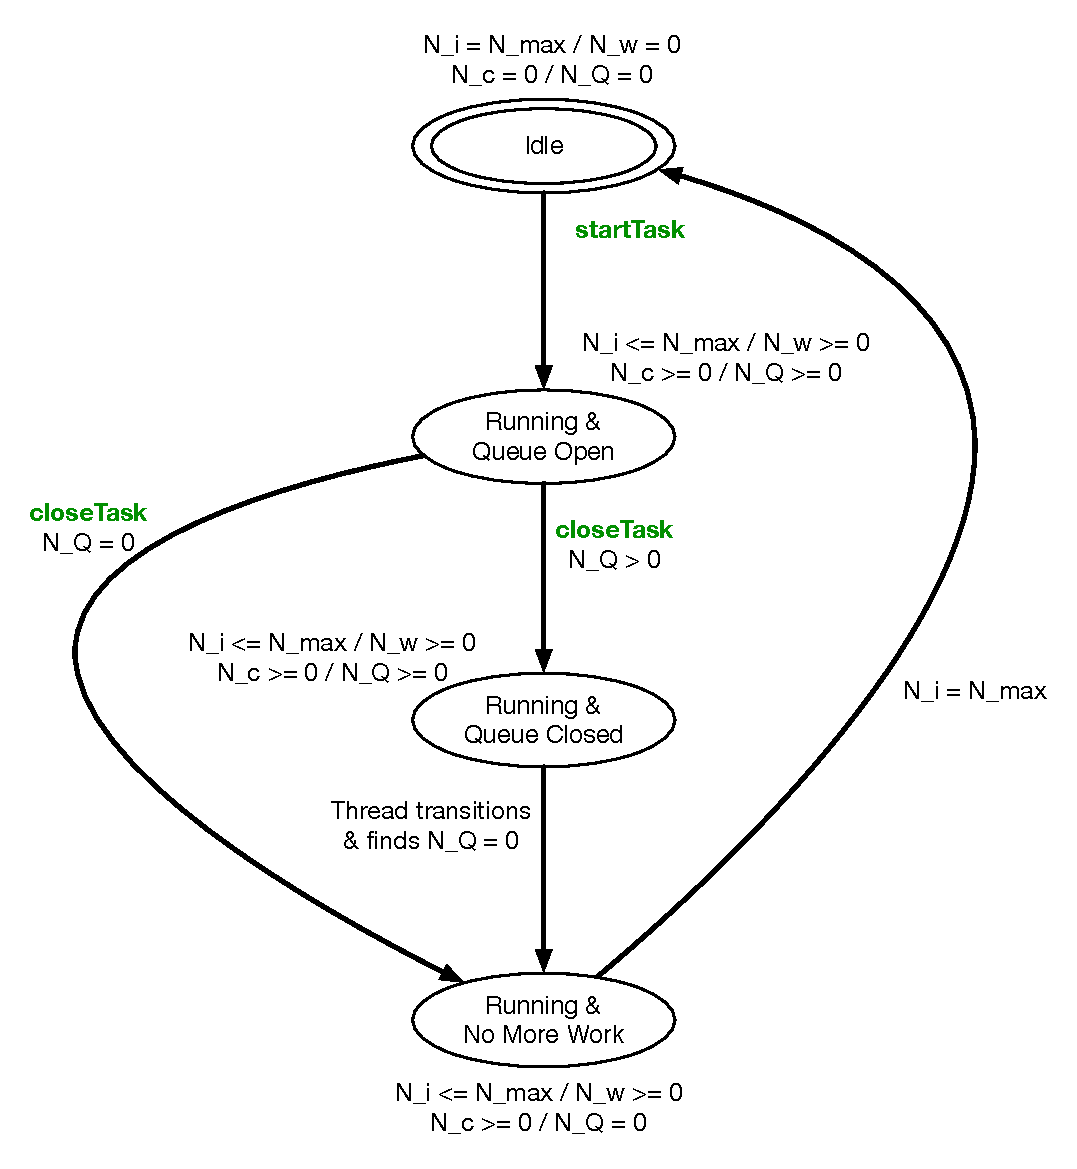
\includegraphics[width=5.0in]{TeamStates.pdf}
\caption[]{}
\label{fig:TeamStateDiagram}
\end{center}
\end{figure}

\begin{figure}[!hp]
\begin{center}
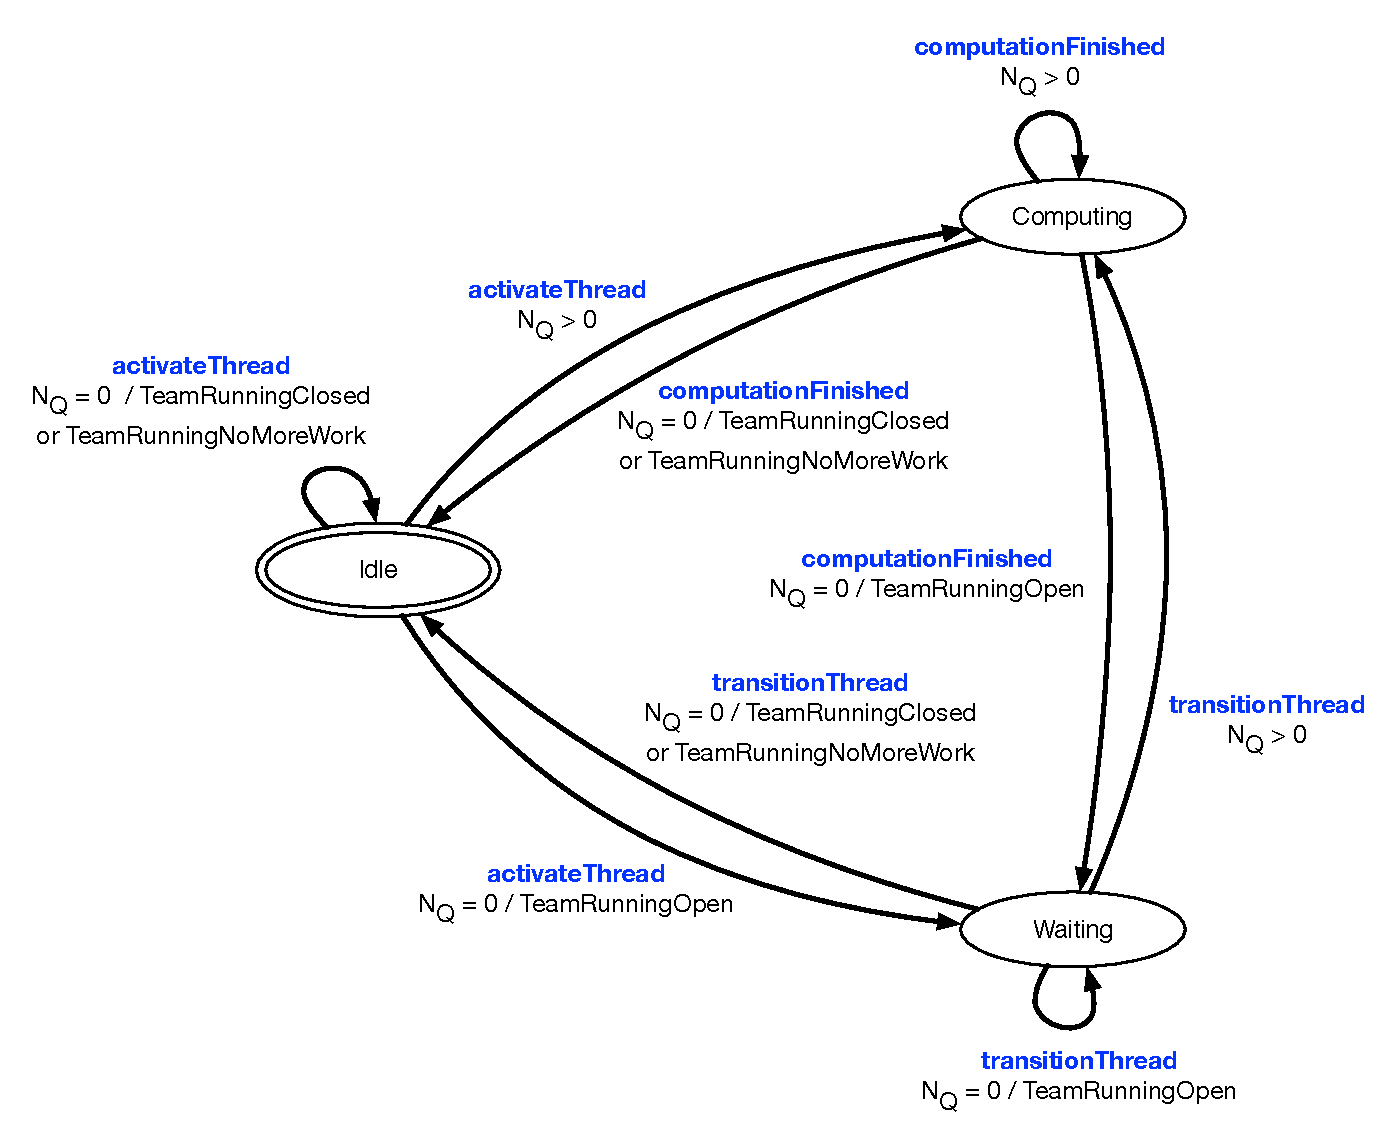
\includegraphics[width=6.5in]{ThreadStatesPersistent.pdf}
\caption[]{}
\label{fig:ThreadStateDiagram}
\end{center}
\end{figure}

\begin{spec}
\label{spec:Runtime_AtomicTransition}
As per the requirements of FSMs, each transition shall be implemented so that
the code executing the transition has sole access to the thread team's state
during the entirety of the transition.  This implies that no other thread can
alter the state simultaneously and that transitions are atomic.
\end{spec}
\textbf{Verification:}\hspace{0.125in}  Each thread team object has a single,
dedicated mutex that must be acquired to access or alter thread team state
information.  Each transition acquires the mutex either through an explicit
request or by a thread receiving an event.  The mutex is not released until
the transition is finalized.\\

Given the present implementation, it is important for transitions that
change the mode and emit internal signals that the code change the mode
\textbf{first} and then emit the signals.  This prevents the possible
(\textbf{TBC} for pthreads?) case that the signal is emitted and received before
the mode is correctly transitioned, which would violate
Spec~\ref{spec:Runtime_AtomicTransition} and cause the responding thread
to react to the signal is a way that is potentially not in accord with the true
mode of the EFSM.

\begin{spec}
A thread team shall maintain a set of pending units of work and all threads in a
thread team shall be able to check the set of pending units of work.  In
addition, each thread in the team shall be able to claim ownership of a single
unit of work by removing it from the set with the understanding that the thread
itself is responsible for applying the team's task to that unit of work.  It
shall be impossible for two threads to simultaneously claim ownership of the
same unit of work.
\end{spec}
\textbf{Verification:}\hspace{0.125in}  Pending work queues implemented as
stated.  As per Spec~\ref{spec:Runtime_AtomicTransition}, dequeueing of units of
work are only done after obtaining the mutex and no handle to dequeued units of
work remain.  Therefore, the only thread that can access a dequeued unit of work
is the thread that dequeued it.
\begin{spec}
All threads that transition to Idle must wait for the \texttt{activateThread}
event.  This includes threads in Idle that receive the \texttt{activateThread}
event but remain in Idle as well as all threads that are \textit{set} into the
Idle state when the EFSM is setup in the initial state.
\label{spec:IdleActivateThread}
\end{spec}

\begin{spec}
External code shall only be able to decrease $N_i$ through the
\texttt{startTask} and \texttt{increaseThreadCount} events and the runtime shall
be implemented such that a request to activate $i$ threads results in an error
if $i$ exceeds the number of Idle threads that are available for activation.
Note that this technical specification is consistent with
Req~\ref{req:ThreadBalance}.
\end{spec}
\textbf{Verification:}\hspace{0.125in}  In the present design, this requirement
is important because the runtime would emit more \texttt{activateThread} signals
than there are threads to receive them.  Because teams allow for thread
publishers/subscribers, undetected signals would amount to a loss of thread
resources at the level of the runtime.  Note that a thread-based implementation
will have a lag between when these events trigger the activation of Idle threads
and when these threads are actually activated.  The runtime design therefore
tracks the actual number of Idle threads with \texttt{N\_idle\_} = $N_i$ as well
as the number of threads pending activation with \texttt{N\_to\_activate\_}.
When a thread does receive \texttt{activateThread}, it decrements both
\texttt{N\_idle\_} and \texttt{N\_to\_activate\_} by one and increments by one
the internal state variable $N_i, N_w$ or $N_c$ corresponding to the thread's
next state.  To satisfy the requirement, both events throw an error if $i > $
\texttt{N\_idle\_} - \texttt{N\_to\_activate\_}.  No other public thread team
methods can emit \texttt{activateThread}.

\begin{spec}
\label{spec:Runtime_OneWait}
The interface of the thread team shall contain a \texttt{wait} method so that
for each task execution, the execution of an external thread that calls
\texttt{wait} is blocked until the termination of the task.  This interface
shall allow for at most one such thread to block its execution with this method
during each task execution.
\end{spec}
\textbf{Verification:}\hspace{0.125in}  Implemented a flag
\texttt{isWaitBlocking\_} to track if a thread has already called \texttt{wait}.

\textcolor{red}{Should we have a variant of wait that accepts a timeout?}

\begin{spec}
To maintain a simple design, client code shall only be allowed to attach and
detach thread subscribers when the team is in the {\TeamIdle} mode.  The same
requirement applies for work subscribers.
\end{spec}
\textbf{Verification:}\hspace{0.125in} Implemented directly as stated.

\begin{spec}
In the original designs, the Team state machine also contained a
{\TeamTerminating} mode.  The transition to this mode was allowed only from
{\TeamIdle} and was triggered by initiating the destruction of the team.  While
sensible, this design was flawed since a runtime error that occurs with the team
in any state could trigger the destruction of the team.  Therefore, the
termination of the EFSM and the clean-up of its resources shall be possible from
any state.
\end{spec}
\textbf{Verification:}\hspace{0.125in}  The destructor does not do any error
checking to confirm that destruction was called with the EFSM in any particular
state.  Also, the destructor assumes that there are Idle, Waiting, and Computing
threads at the time of calling.  For the Idle and Waiting threads, it signals 
them to terminate; Computing threads, it waits for them to finish their work and
discover that they should terminate.

\begin{spec}
\label{spec:Runtime_AwakenOnNoMoreWork}
All transitions to {\TeamRunningNoMoreWork} from a different mode shall awaken
all Waiting threads so that they can transition to Idle.
\end{spec}
\textbf{Verification:}\hspace{0.125in}  Implemented directly as stated.

\begin{spec}
\label{spec:Runtime_CompMustEnqueue}
Upon emitting/receiving the \texttt{computationFinished} signal, a Computing
thread shall enqueue the unit of work that it just finished applying the team's
task to with the team's work subscriber if the team has a work subscriber.
\end{spec}
\textbf{Verification:}\hspace{0.125in}  Implemented directly as stated.

\begin{spec}
\label{spec:Runtime_IdleOutput}
All transitions to {\TeamIdle} from a different mode shall
\begin{itemize}
\item{call the \texttt{closeTask} method of the team's work subscriber if it
has a work subscriber and }
\item{unblock the external thread that called \texttt{wait} if such a thread
exists.}
\end{itemize}
If the transition to {\TeamIdle} is handled by a Computing thread, then the
Computing thread shall enqueue its unit of work
(Spec~\ref{spec:Runtime_CompMustEnqueue}) prior to calling \texttt{closeTask}.
Note that this specification is not applicable to the case of \textit{setting}
the EFSM into its initial state.
\end{spec}
\textbf{Verification:}\hspace{0.125in}  Implemented directly as stated.

\begin{spec}
\label{spec:Runtime_IdleToIdle}
It is possible for an Idle thread to receive the \texttt{activateThread} event
when the team does not need threads to be activated (\textit{i.e.} the mode is
\TeamIdle \footnote{Consider a team that is both a thread publisher and
subscriber.  It is possible for the team to finish its work and transition to
{\TeamIdle} before its publisher and subscriber finish their work.} or
\TeamRunningNoMoreWork).  To avoid thread resource loss and to promote efficient
execution of the execution cycle's tasks, in this scenario the threads that
receive the unnecessary event shall remain in Idle and call
\texttt{increaseThreadCount(1)} for its thread subscriber if it exists.
\end{spec}
\textbf{Verification:}\hspace{0.125in} Implemented directly as stated.

\begin{spec}
\label{spec:Runtime_ForwardThreads}
To prevent thread resource loss at the level of the runtime, all threads that
transition to Idle shall call \texttt{increaseThreadCount(1)} of its thread
subscriber should it exist.  This specification is consistent with
Spec~\ref{spec:Runtime_IdleToIdle}, which could be understood to handle the
special case that an Idle thread transitions to Idle.  Note that this
specification is not applicable to the case of \textit{setting} the EFSM into
its initial state.  Note that this technical specification is consistent with
Req~\ref{req:ThreadSubPub}.
\end{spec}
\textbf{Verification:}\hspace{0.125in} Implemented directly as stated.

\begin{spec}
\label{spec:Runtime_NoEnqueue}
Client code shall only be allowed to give a team a unit of work if the team is
in the mode {\TeamRunningOpen}.  While the runtime could allow clients to give
units of work to a team that is in {\TeamIdle} with the understanding that the
work would be for the next task to be given to the team, there is no known use
case for which this is necessary.  Therefore, this specification is motivated by
the goal of simplifying the design.
\end{spec}
\textbf{Verification:}\hspace{0.125in}  The \texttt{enqueue} method is the only
means for giving a unit of work to a team.  Attempts to use this method when the
team is not in {\TeamRunningOpen} result in error.\\

Based on this specification, client code should call \texttt{startTask} on all
thread teams to be used on a task before enqueueing work with any of these.  This
practice will help avoid the case where an active work publisher tries to
enqueue work on a work subscriber that is still in the mode \TeamIdle.\\

As a final note, the design accounts for \texttt{transitionThread} events that
occur when no Waiting threads exist.  For each of these, this occurrence is
acceptable and no output is generated as part of the transition.  This
transition is included for the sake of completeness and can occur with the
current implementation when certain outputs broadcast \texttt{transitionThread}.
Unlike for \texttt{activateThread}, it is unimportant that there is no thread to
receive the event.  This is due to the fact that this event exists to inform a
Waiting thread to look for work or that it should determine that it should
transition to Idle.  If there are no Waiting threads because all threads are
Idle, then the team must be in \TeamIdle, in which case we don't need to
activate threads, or in \TeamRunningOpen.  In the latter case, we wait for
threads to be activated or for \texttt{closeTask} to be called to transition
the team to \TeamIdle.  If all threads are Computing, then these will discover
that there is pending work and the team will stay maximally busy.

%%-- TEAM IDLE SUBSECTION
\subsubsection{{\TeamIdle} State}
\begin{spec}
Similar to Spec~\ref{spec:Runtime_ForwardThreads}, if client code calls the
\texttt{increaseThreadCount} method of a thread team in \TeamIdle, the team shall
forward the pushed thread resources immediately on to its thread subscriber if
it exists.
\end{spec}
\textbf{Verification:}\hspace{0.125in}  Implemented directly as stated.

\begin{spec}
In the {\TeamIdle} mode, the queue shall always be empty with all threads in the
team in the Idle state.  This implies that no thread can be in the Waiting
state, the Computing state, or terminating and that all threads are therefore
(Spec~\ref{spec:IdleActivateThread}) waiting to receive the
\texttt{activateThread} event.
\end{spec}
\textbf{Verification:}\hspace{0.125in}  The initial state starts in {\TeamIdle}
and specifies that there is no work in the queue.  Also, all transitions to
{\TeamIdle} only happen if the queue is empty.  Therefore, the pending work
queue is always empty upon entry to \TeamIdle.  Finally, no work can be added to
the queue in the {\TeamIdle} state by Spec~\ref{spec:Runtime_NoEnqueue}.\\

The initial state specifies that all threads are Idle and transitions to
{\TeamIdle} only happen if the same is true.  Therefore, the claim is true upon
entry to {\TeamIdle} and all threads are waiting for \texttt{activateThread}.
Also, responses
\footnote{These cases are being considered should one of these
events be emitted when the team in not Idle, but is received after transitioning
to Idle.  With the current implementation, since all threads would be waiting on
\texttt{activateThread}, no threads would be waiting for the latter two events.}
to \texttt{activateThread}, \texttt{transitionThread}, and
\texttt{computationFinishes} do not transition the thread state and have the
responding threads wait for \texttt{activateThread}.  Therefore any attempt to
transition a thread terminates with the thread in Idle.

\begin{spec}
It would seem to be sensible to insist that an external thread cannot call
\texttt{wait} for a team that is in \TeamIdle.  However, it is possible that a
runtime execution cycle could finish and transition a team back to {\TeamIdle}
before an external thread has the chance to call \texttt{wait}.  Therefore, the
\texttt{wait} method shall be enabled in {\TeamIdle} and shall terminate immediately to avoid
unnecessary blocking of the calling thread.  Note that this does allow for
client code to superfluously call \texttt{wait} before the first execution cycle
is run and multiple times between cycles, both of which are logical errors.
\end{spec}
\textbf{Verification:}\hspace{0.125in}  Implemented directly as stated and in
accord with Spec~\ref{spec:Runtime_OneWait}.  

%%-- TEAM RUNNING & OPEN SUBSECTION
\subsubsection{\TeamRunningOpen}
\begin{spec}
It  would seem sensible to insist that an external thread cannot call
\texttt{wait} during a given execution cycle unless the \texttt{closeTask} event
has already been issued for the same cycle.  However, consider the case of two
teams, one of which is the work publisher for the other.  As per
Spec~\ref{spec:Runtime_IdleOutput}, when the publisher team transitions to
{\TeamIdle}, it calls the subscriber's \texttt{closeTask} method to inform the
subscriber that it will not be given more work.  This implies that the external
thread that triggers an execution cycle with the runtime does not know when
\texttt{closeTask} is called and therefore could call \texttt{wait} before this
event occurs.  Hence, a thread team in the state {\TeamRunningOpen} shall allow
for a thread to call \texttt{wait}.
\end{spec}
\textbf{Verification:}\hspace{0.125in}  Implemented directly as stated.

%%-- TEAM RUNNING & CLOSED SUBSECTION
\subsubsection{\TeamRunningClosed}
\begin{spec}
\label{spec:Closed_Transition}
If a team is in mode \TeamRunningClosed, then every thread that transitions to
Computing shall check if $N_Q = 0$ as part of the transition and after
dequeueing the unit of work on which it will apply its team's task.  If $N_Q =
0$, then during the same transition (and therefore before applying the task to
the dequeued unit of work) the thread shall change the mode to
\TeamRunningNoMoreWork.
\end{spec}
\textbf{Verification:}\hspace{0.125in}  A thread can be transitioned to
Computing from the Idle, Waiting, and Computing state.  If the mode is
{\TeamRunningClosed}, $N_Q = 1$, and a
thread receives any of the \texttt{activateThread}, \texttt{transitionThread},
or \texttt{computationFinished} events, then the induced transitions always changes
the mode to \TeamRunningNoMoreWork.  No other events result in decreasing $N_Q$
to zero in \TeamRunningClosed.

\begin{spec}
\label{spec:Closed_NoWork}
The transition from {\TeamRunningClosed} to \TeamRunningNoMoreWork, which is the
only transition possible for this mode, is triggered internally by the active
thread that dequeues the last unit of work (Spec~\ref{spec:Closed_Transition}).
Therefore, to avoid deadlock the design of the runtime shall be such that the
EFSM cannot be in mode {\TeamRunningClosed} with $N_Q = 0$.  Note that it is not
necessarily an error if $N_i = N_{max}$ in {\TeamRunningClosed} as the team
could be a thread subscriber and have a thread activated by its publisher so
that the team could eventually dequeue elements and determine that there is no
more work.
\textcolor{red}{Should each thread team store the pointer to its thread
publisher so that we can implement a rule here that if a team isn't a thread
subscriber and $N_i = N_{max}$, then we have an error?}
\end{spec}
\textbf{Verification:}\hspace{0.125in}  The only transition to
{\TeamRunningClosed} is from {\TeamRunningOpen}, which only occurs if $N_Q > 0$.
Hence, the specification is satisfied upon entry into the mode.  The value of
$N_Q$ can decrease in this mode only when a thread transitions to the Computing
state.   By Spec~\ref{spec:Closed_Transition}, the EFSM mode is transitioned to
{\TeamRunningNoMoreWork} as part of every transition that results in $N_Q = 0$.

%%-- TEAM RUNNING & NO MORE WORK SUBSECTION
\subsubsection{\TeamRunningNoMoreWork}
For the following, note that the only transitions into {\TeamRunningNoMoreWork}
are from {\TeamRunningOpen} and \TeamRunningClosed.

\begin{spec}
\label{spec:NoMoreWork_NoWork}
If a team is in \TeamRunningNoMoreWork, then it shall always be true that $N_Q =
0$.
\end{spec}
\textbf{Verification:}\hspace{0.125in}  
Since both transitions into {\TeamRunningNoMoreWork} only occur if $N_Q = 0$,
the specification is satisfied upon entry to the mode.  The only means to
increase $N_Q$ is by adding work \textit{via} \texttt{enqueue}, which is
prohibited in {\TeamRunningNoMoreWork} by Spec~\ref{spec:Runtime_NoEnqueue}.

\begin{spec}
\label{spec:NoMoreWork_TransitionToIdle}
If a team is in mode \TeamRunningNoMoreWork, then the last thread to transition
to Idle shall change the mode to \TeamIdle.  This transition is valid as $N_i =
N_{max}$ necessarily at the transition and by Spec~\ref{spec:NoMoreWork_NoWork}
it is certain that $N_Q = 0$.
\end{spec}
\textbf{Verification:}\hspace{0.125in}  If the transition to
{\TeamRunningNoMoreWork} is from \TeamRunningOpen, then $N_w > 0$ or $N_c > 0$
(to the contrary, $N_Q = 0$ and $N_i = N_{max}$ so that the transition is to
\TeamIdle).  If the transition is from \TeamRunningClosed, then it follows from
Spec~\ref{spec:Closed_Transition} that $N_c > 0$.  Therefore, upon entry to the
mode, there is at least one thread that could transition to Idle.  Since
satisfaction of Spec~\ref{spec:NoMoreWork_NoWork} implies that $N_Q = 0$, all
Computing threads will determine upon finishing the application of the team's
task to the current unit of work that there is no more work and will
subsequently transition to Idle.  Similarly, satisfaction of
Spec~\ref{spec:Runtime_AwakenOnNoMoreWork} implies that all threads in the Wait
state will be awakened, determine that there is no work, and transition to Idle
as well.  Therefore, all non-active threads will eventually transition to Idle.
Given this and the fact that the reception of \texttt{activateThread} events are
effectively ignored by Idle threads, we conclude that there will be a last
thread that transitions to Idle.  This thread is programmed to transition the
mode to \TeamIdle.

\begin{spec}
\label{spec:NoMoreWork_NeedThread}
The transition from {\TeamRunningNoMoreWork} to \TeamIdle, which is the only
transition out of this mode, occurs when the last non-Idle thread transitions to
Idle (See Spec~\ref{spec:NoMoreWork_TransitionToIdle}).  Therefore, to avoid
deadlock the design of the runtime shall prohibit the EFSM from being in a state
with {\TeamRunningNoMoreWork} and $N_i = N_{max}$.
\end{spec}
\textbf{Verification:}\hspace{0.125in} As shown in the Verification of
Spec~\ref{spec:NoMoreWork_TransitionToIdle},  $N_i < N_{max}$ upon entry to the
mode.  As $N_i$ can only decrease by at most one with each thread transition,
which are atomic (Spec~\ref{spec:Runtime_AtomicTransition}), satisfaction of
Spec~\ref{spec:NoMoreWork_TransitionToIdle} implies that $N_i$ cannot be set to
zero in {\TeamRunningNoMoreWork} without also simultaneously causing the mode to
change to \TeamIdle.  Hence, $N_i < N_{max}$ in {\TeamRunningNoMoreWork} up to
the transition to \TeamIdle.

%\subsection{Possible Requirements}
%If a thread team is going to ship data to an accelerator like a GPU, then the
%unit of work for such a thread team shall be a data packet of tiles (with the
%possibility that the tiles are the trivial tiling).  This includes the
%possibility of data packets that consist of a single tile (and therefore tile
%that consist of a single block). 

%If a thread team is going to ship data to the host, then the unit of work for
%such a thread team shall be a tile (with the possibility that the tiles are the
%trivial tiling).

%Consider a unit of runtime work that includes a GPU-concurrent task, a
%CPU-concurrent task, and a Post-concurrency CPU task in its task bundle.  Then
%for each block in a data packet, the concurrent CPU task will have blocks of
%input data (CC, FC[XYZ], Fluxes[XYZ], etc.), output data (CC, FC[XYZ],
%Fluxes[XYZ], etc.), and scratch blocks (e.g. grav[XYZ], auxC).  The concurrent
%GPU task will have the same, but non-intersecting block structure.  The
%post-concurrency CPU task can use whatever is in MFabs that is not being worked
%on by the concurrent CPU task and can allocate its own CPU scratch blocks.  We
%can get the CPU scratch memory through the runtime memory manager, but I don't
%know if we need to manage that memory or just let failures happen.  This assumes
%that the host memory will never be the limiting memory pool factor (i.e. that
%the host memory will always be much larger than the device memory).\\

%It is possible that certain units of runtime work will not need to bring the
%data back to the host memory as that same data is needed by the next runtime
%execution in the same device.  However, since we cannot assume that all the
%memory will fit in the device memory, we must assume that in the worst case only
%a fraction of the intended blocks will stay in the device memory.  The runtime
%shall maintain location information for each block that persists across calls to
%the runtime.  When the next runtime execution begins, those blocks already in
%the device shall be grouped into one or more data packets and work immediately
%launched on these.  The runtime shall not include these same blocks in a
%subsequent data packet so that we avoid repeated work.  FLASH shall abort
%execution if, at the end of a time step, we have blocks of persistent data
%(\textit{e.g.} unk) that are not in the host memory.  \textcolor{red}{Are these
%really requirements that we want?  If yes, then the blocks in the device memory
%would be the first data packet and therefore we get the pipeline up and running
%quicker.}  Example of this is unsplit Hydro.  The computeFluxes routine pulls in
%the UNK data on CC1 and updates the fluxes.  Neither needs to go back to the GPU
%ever.  The updated solution is in CC2.  Note that if we have the future case of
%host and some devices sharing the same physical memory, this requirement could
%become more imporatant.  Therefore, giving the runtime more parameters to inform
%data movements could be important.\\

%Should we allow the Post-concurrency task to start immediately when blocks get
%back from the GPU?  This would imply that this task is also independent from the
%CPU-concurrent task.  Or, do we run the Post-concurrent task only after both the
%CPU and GPU work have finished?  Note that we can never know that a single
%routine will always run on either the host or either the device.  They must be
%written in such a way that they can be run well on either without manual or
%automatically updating the code beyond directives (OpenACC, OpenMP, CUDA, etc.).\\

%\newpage
%\begin{appendices}
%\section{Hydro operations}
%The Unsplit implementation of the Hydro step operation has at least three
%variants and the variant executed at runtime is presently determined at each
%time step based on the Grid unit AMR implementation chosen (known at setup) 
%and whether or not flux correction should be applied (specified as a runtime
%parameter).  Here we express each variant as an operation.\\
%
%\textcolor{red}{TODO: Add to requirements that parameter such as flux correction
%should be both a setup and runtime parameter.  If the setup-time value is false,
%then the task scheduler has the possibility to fuse tasks.  If it is true, then
%the runtime parameter can still be set to turn this off.  However, the binary
%built will not have been built with the potential for fusing tasks.}\\
%
%For the following subsections, the colorization is
%\begin{itemize}
%\item{a \ComposerKey{keyword} that is paired with a static Fortran routine in
%the operation's dictionary,}
%\item{a \RuntimeParam{runtime} parameter, and}
%\item{a \SetuptimeParam{setup-time} and runtime parameter.}
%\end{itemize}
%
%TODO: Add in a UG variant?!
%
%\newpage
%\subsection{No flux correction variant}
%\texttt{
%\begin{tabbing}
%\hspace*{0.25in}\=\hspace*{0.25in}\= \kill
%if \SetuptimeParam{shockDetectOn}:\\
%\>\ComposerKey{GcFillWithoutEoS} (global, internode data movement)\\
%\> Task 1:\\
%\>\> \ComposerKey{doShockDetection}\\
%\ComposerKey{GcFillWithEoS} (global, internode data movement)\\
%Task 2:\\
%\> if \RuntimeParam{updateHydroFluxes}:\\
%\>\> \ComposerKey{updateHydroData}\\
%\> \ComposerKey{zeroFluxData}\\
%\> iterate \ComposerKey{LeavesWithoutTiling}:\\
%\>\> \ComposerKey{computeFluxesAndUpdateSolution}\\
%\end{tabbing}
%}
%
%For \ComposerKey{computeFluxesAndUpdateSolution}, the dictionary should know
%that it needs to run \texttt{hy\_computeFluxes} with \texttt{Uout => Uin}.
%
%\subsection{Paramesh + flux correction variant}
%\texttt{
%\begin{tabbing}
%\hspace*{0.25in}\=\hspace*{0.25in}\=\hspace*{0.25in}\= \kill
%if \SetuptimeParam{shockDetectOn}:\\
%\>\ComposerKey{GcFillWithoutEoS} (global, internode data movement)\\
%\> Task 1:\\
%\>\> \ComposerKey{doShockDetection}\\
%\ComposerKey{GcFillWithEoS} (global, internode data movement)\\
%Task 2:\\
%\> if \RuntimeParam{updateHydroFluxes}:\\
%\>\> \ComposerKey{updateHydroData}\\
%\> \ComposerKey{zeroFluxData}\\
%\> iterate \ComposerKey{LeavesWithoutTiling}:\\
%\>\> if level == finest:\\
%\>\>\> \ComposerKey{computeFluxesAndUpdateSolution}\\
%\>\> else:\\
%\>\>\> \ComposerKey{computeFluxes}\\
%\> \ComposerKey{storeFluxDataForFluxCorrect}\\
%\ComposerKey{conserveFluxes} (global, internode data movement)\\
%Task 3:\\
%\> iterate \ComposerKey{LeavesWithoutTiling}:\\
%\>\> if level == finest:\\
%\>\>\> \ComposerKey{noOp}\\
%\>\> else:\\
%\>\>\> \ComposerKey{updateSolution}\\
%\> \ComposerKey{updateBoundaries}
%\end{tabbing}
%}
%
%\newpage
%\subsection{AMReX + flux correction variant - tiling}  
%\textbf{Input:} \texttt{simTime, dt, dtOld, sweepOrder}\\
%\textbf{Output:} the updated solution with EoS run on all leaf blocks.  GC data
%not necessarily good.
%
%\texttt{
%\begin{tabbing}
%\hspace*{0.25in}\=\hspace*{0.25in}\=\hspace*{0.25in}\=\hspace*{0.25in}\= \kill
%if \SetuptimeParam{shockDetectOn}:\\
%\>\ComposerKey{GcFillWithoutEoS} (global, internode data movement)\\
%\> Task 1:\\
%\>\> iterate \ComposerKey{LeavesOnLevelWithoutTiling}:\\
%\>\>\> \ComposerKey{doShockDetection} (operates on single block)\\
%\ComposerKey{GcFillWithEoS} (global, internode data movement)\\
%Task 2:\\
%\> if \RuntimeParam{updateHydroFluxes}:\\
%\>\> SubTask 2.1 (Run in device so that data is already in device memory?):\\
%\>\>\> \ComposerKey{updateHydroData} (doesn't operate on blocks, but sets
%variables)\\
%\> SubTask 2.2 (Run in CPU to avoid data movements?):\\
%\>\> \ComposerKey{zeroFluxData} (iterates over all leaf blocks)\\
%\ComposerKey{TaskBarrier} (fake data movement so that tasks are clean and efficient)\\
%Task 3:\\
%\> level = finest\\
%\> iterate \ComposerKey{LeavesOnLevelWithoutTiling}:\\
%\>\> \ComposerKey{computeFluxesAndUpdateSolution}\\
%\> if \ComposerKey{nLevels} > 1:\\
%\>\> \ComposerKey{storeFluxDataForFluxCorrect}\\
%\> level = finest-1 (NOTE: There might only be one level at any iteration!)\\
%\> iterate \ComposerKey{LeavesOnLevelWithoutTiling}:\\
%\>\> \ComposerKey{computeFluxes}\\
%\> if level != coarsest:\\
%\>\> \ComposerKey{storeFluxDataForFluxCorrect}\\
%\ComposerKey{conserveFluxes} (global, internode data movement)\\
%loop level=finest-1..coarsest:\\
%\>Task 3+i:\\
%\>\> iterate \ComposerKey{LeavesOnLevelWithoutTiling}:\\
%\>\>\> \ComposerKey{updateSolution}\\
%\>\> level = finest-i\\
%\>\> iterate \ComposerKey{LeavesOnLevelWithoutTiling}:\\
%\>\>\> \ComposerKey{computeFluxes}\\
%\>\> if level != coarsest:\\
%\>\>\> \ComposerKey{storeFluxDataForFluxCorrect}\\
%\ComposerKey{conserveFluxes} (global, internode data movement)\\[0.25in]
%Task M:\\
%if \SetuptimeParam{useGravity}:\\
%\> \ComposerKey{prepareNewGravityAccelerations}\\
%\ComposerKey{doGravityStep}
%\ComposerKey{TaskBarrier} (Implied because we are at the end of the operation?)
%\end{tabbing}
%}
%
%Note that \texttt{hy\_updateSolution} calls \texttt{hy\_energyFix} and \texttt{Eos\_wrapped}
%at the end.  These two could be pulled out and included as subtasks that could
%be run on the CPU after \texttt{hy\_updateSolution} finishes running on a data
%packet in the accelerator.\\
%
%Note that \texttt{hy\_prepareNewGravityAccelerations} can call
%Gravity\_potential and GcFill in the end.  This needs to be moved up.\\
%
%Note that \texttt{hy\_gravityStep} iterates over all leaf blocks to update the
%solution using the gravity accelerations.
%
%\end{appendices}

\end{document}
